
\section{Observables and Kinematic Discriminants}
\label{sec:observables}

Several observables, such as the four-lepton invariant mass, $m_{4\ell}$, or the kinematic discriminants,
are used either as input to likelihood fits or to categorize events in this analysis. 

%======================================================

\subsection{Description of discriminant setup and algorithms}

The full kinematic information from each event using either the Higgs boson decay or associated
particles in its production is extracted using the matrix element calculations. 
These discriminants use a complete set of mass and angular
input observables $\vec\Omega$~\cite{Gao:2010qx,Anderson:2013afp,Gritsan:2016hjl} 
to describe kinematics at LO in QCD, see Fig.~\ref{fig:decay}.
The \PT of either the combined \PH boson and 2 jets system for the production discriminant
(e.g. $\mathcal{D}_{\rm 2jet/1jet/VH}$)~\cite{Khachatryan:2015cwa, Khachatryan:2015mma} 
or the \PH boson itself for the decay 
discriminants (e.g. $\mathcal{D}^{\rm kin}$)~\cite{Chatrchyan:2012ufa,Khachatryan:2014kca}
is not included in the input observables in order to reduce associated QCD uncertainties. 

%%%%%%
The kinematic discriminants used in this study are computed using the {\sc MELA}
package~\cite{Chatrchyan:2012ufa,Gao:2010qx,Bolognesi:2012mm,Anderson:2013afp},
which provides the full set of processes studied in this paper and uses \textsc{JHUGen} matrix elements
for the signal and \MCFM matrix elements for the background. The signal includes both 
the four-lepton decay kinematics in the processes  $\Pg\Pg$ or 
$q\bar{q}\to X\to \Z\Z$ / $\Z\gamma^*$ / $\gamma^*\gamma^*\to4\ell$, and kinematics of
associated particles in production $H$+jet, $H$+2jets, VBF, $\Z\PH$, $W\PH$, $t\bar{t}H$, $tqH$, or $b\bar{b}H$. 
The background includes $\Pg\Pg$ or $q\bar{q}\to\Z\Z$ / $\Z\gamma^*$ / $\gamma^*\gamma^*$ / $\Z\to 4\ell$
processes. 
Additional algorithms are available for the cross-checks of the four-lepton kinematics in decay. 
Within the {\sc MELA} framework, an analytic parameterization of the matrix elements
for signal~\cite{Gao:2010qx,Bolognesi:2012mm} and background~\cite{Chen:2012jy} was adopted in the previous CMS
analyses, reported in Refs.~\cite{Chatrchyan:2012ufa,Chatrchyan:2013lba,Chatrchyan:2012jja}, and is used for
cross-checks in this analysis. 
The four-lepton matrix element calculations are also tested
with the \textsc{mekd} package~\cite{Avery:2012um}, which is based on \MADGRAPH
and \textsc{FeynRules}~\cite{Christensen:2008py}, for a subset of four-lepton decay 
processes implemented in common with {\sc MELA}.

%%=============
\begin{figure}[!htb]
%\vspace*{0.3cm}
\begin{center}
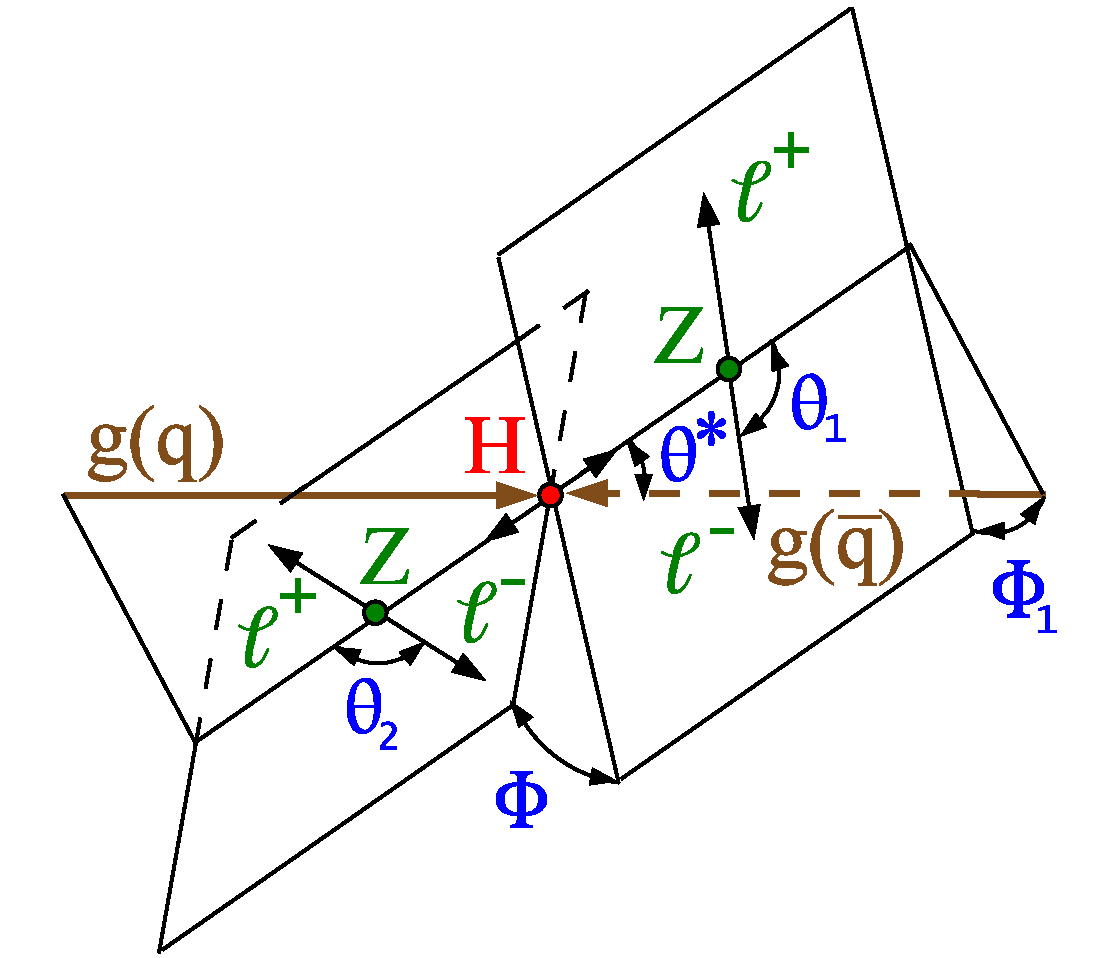
\includegraphics[width=0.45\textwidth]{Figures/Observables/angles-h4l.pdf}
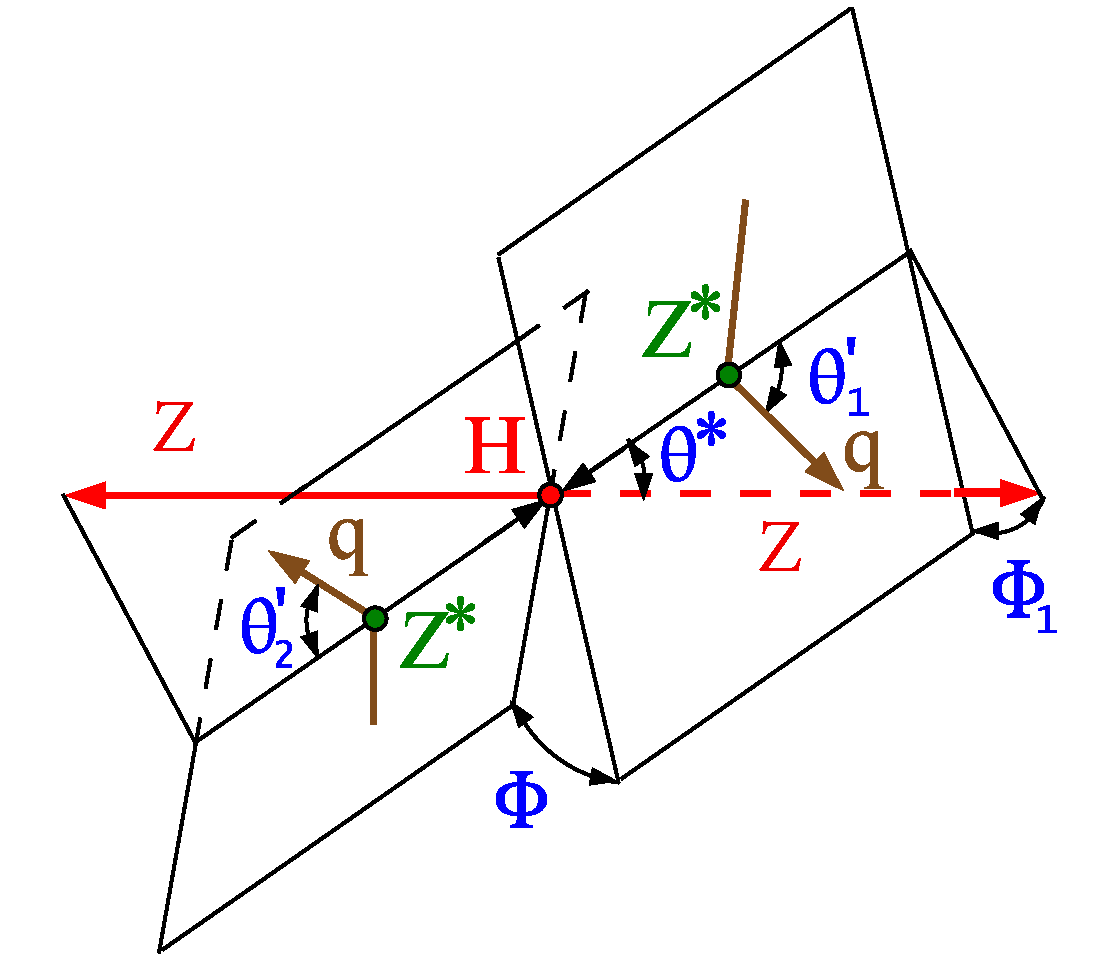
\includegraphics[width=0.45\textwidth]{Figures/Observables/angles-vbf.pdf}
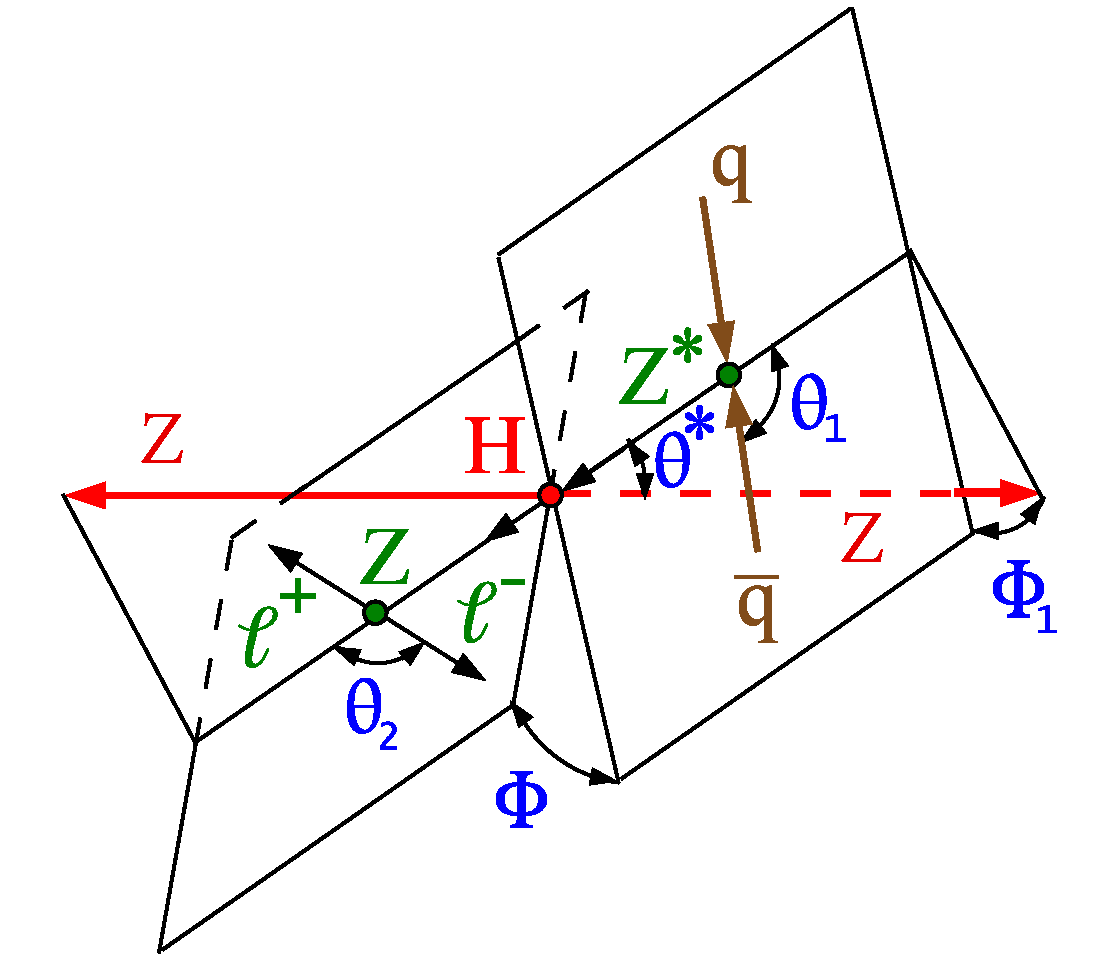
\includegraphics[width=0.45\textwidth]{Figures/Observables/angles-vh.pdf}
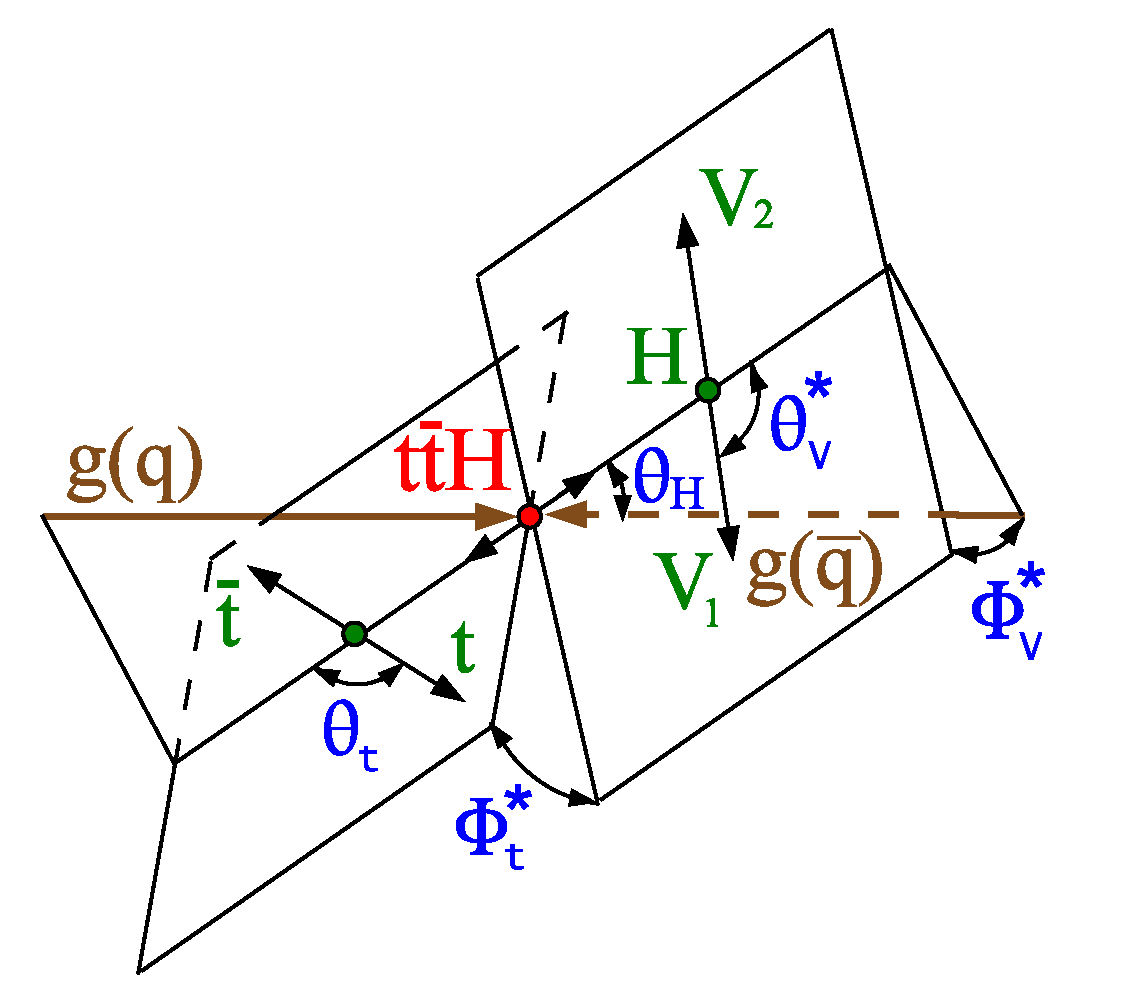
\includegraphics[width=0.45\textwidth]{Figures/Observables/angles-tth1.pdf}
\caption
{ 
Illustrations of $\PH$ particle production and decay 
$gg/q\bar{q}\to \PH\to ZZ\to 4\ell^\pm$ (top-left),
VBF $q{q^\prime}\to q{q^\prime} \PH$ (top-right),
$q\bar{q}\to V^*\to VH$ (bottom-left), and
$gg/q\bar{q}\to t\bar{t} \PH$ (bottom-right).
Angles and invariant masses fully characterize the orientation of the production and decay chain and are defined 
in the suitable rest frames~\cite{Gao:2010qx,Anderson:2013afp,Gritsan:2016hjl}.
\label{fig:decay}
}
\end{center}
\end{figure}
%%=======

%================================================

\subsection{Description of kinematic discriminants}
\label{sec:kindistr}

\subsubsection{Kinematic discriminants for final fit}
The discriminant sensitive to the $\Pg\Pg/q\bar{q}\to4\ell$ kinematics is calculated as~\cite{Chatrchyan:2012ufa,Khachatryan:2014kca} 
%%%%%%%%%%%%%%%%%%%%%
\begin{eqnarray}
%
\label{eq:ggmela}
\mathcal{D}^{\rm kin}_{\rm bkg} = 
\left[1+  \frac{ \mathcal{P}^{\Pq \Paq }_\text{bkg} (\vec\Omega^{\PH\to4\ell} | m_{4\ell})  }
{ \mathcal{P}^{\cPg\cPg}_\text{sig}(\vec\Omega^{\PH\to4\ell} | m_{4\ell}) } \right]^{-1}\,,
%
\end{eqnarray}
%%%%%%%%%%%%%%%%%%%%%
where the denominator contains the probability for the signal 
and the numerator includes the probability for the dominant $q\bar{q}\to4\ell$ background process, 
all calculated either with the 
\textsc{JHUGen} or \MCFM matrix elements within the MELA framework.
Figure~\ref{fig:dbkgkin} shows conditional distribution of $\mathcal{D}^{\rm kin}_{\rm bkg}$ for signal and background as a function of $m_{4\ell}$, in the Untagged category.
% $q\bar{q}\to 4\ell$ background as a function of $m_{4\ell}$.

%=======
\begin{figure}[!htb]
\vspace*{0.3cm}
\begin{center}
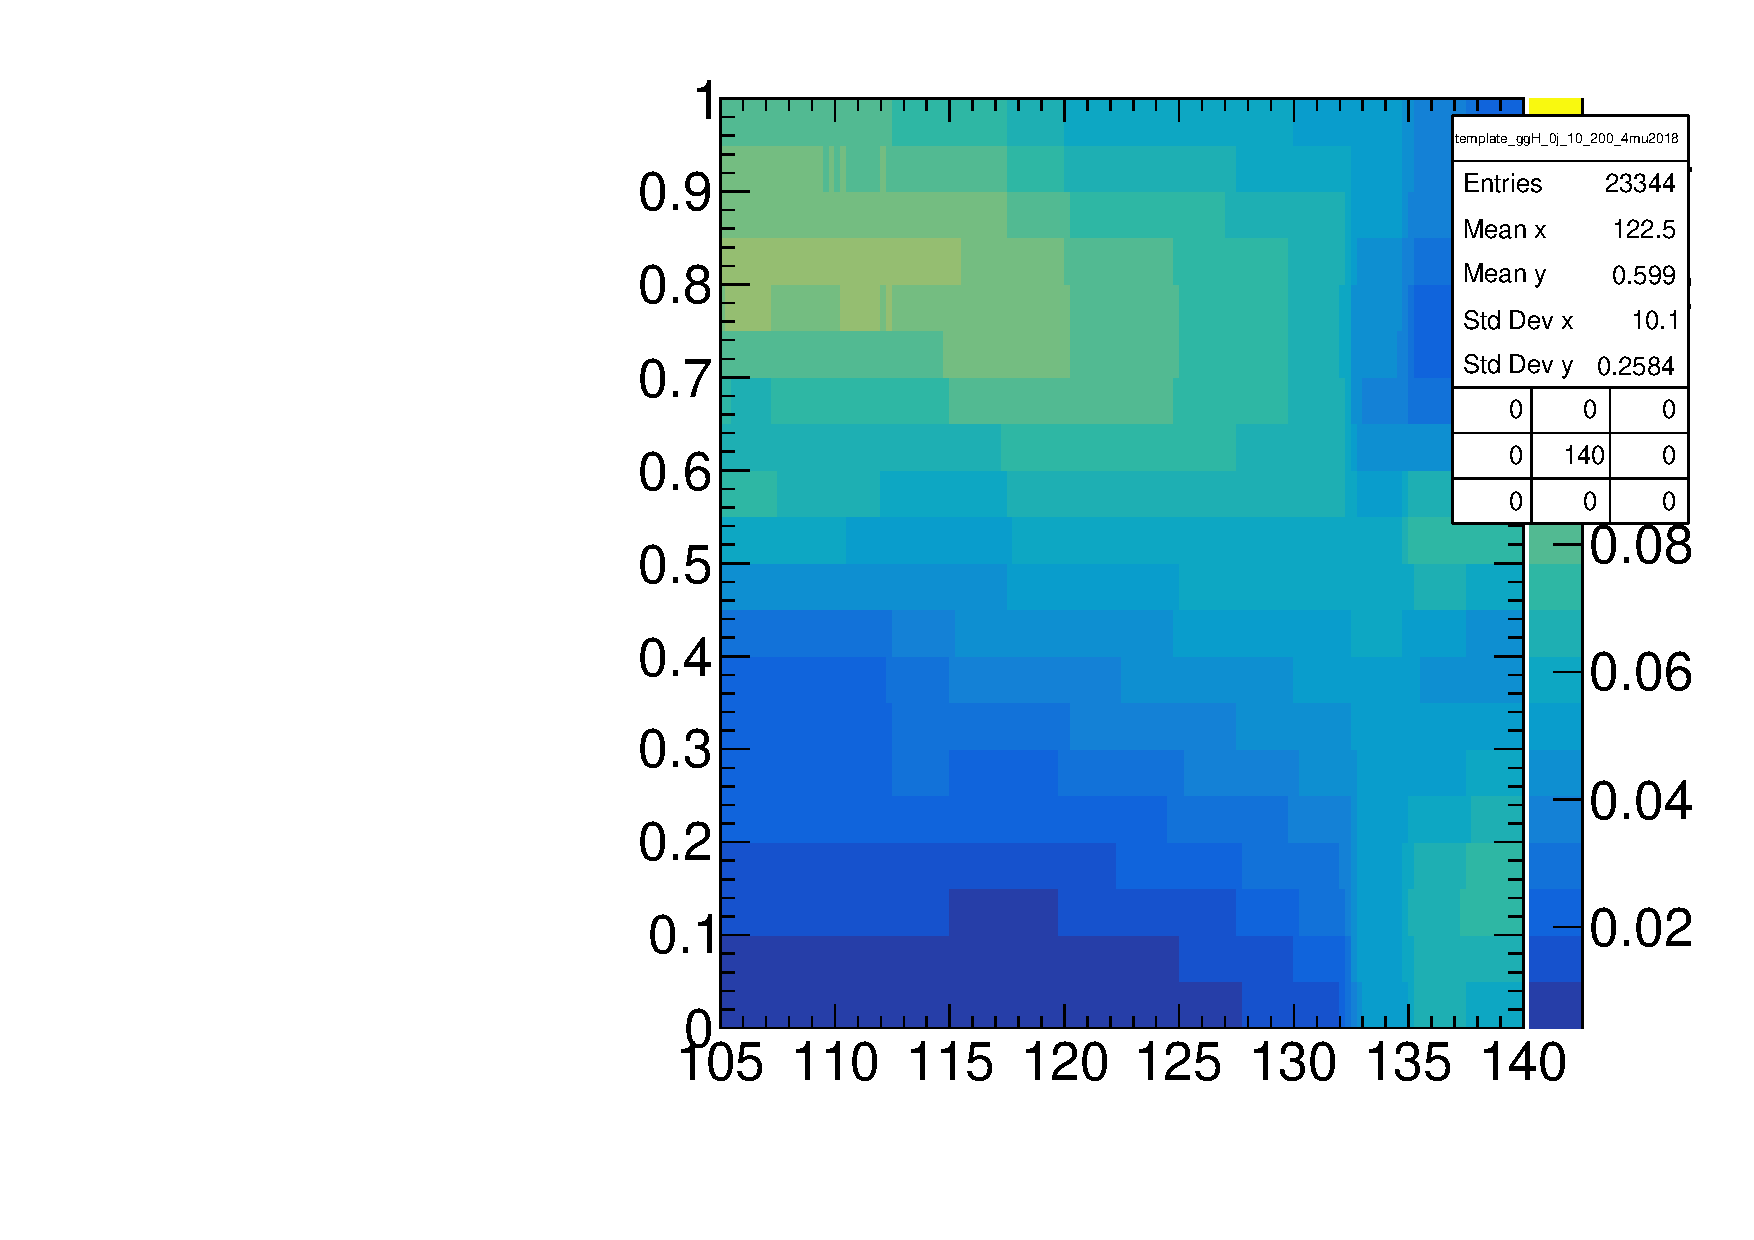
\includegraphics[width=0.45\textwidth]{Figures/Observables/template_ggH_0j_10_200_4mu2018template.pdf}%Observables/Templates_4mu_Untagged_ggH.pdf}
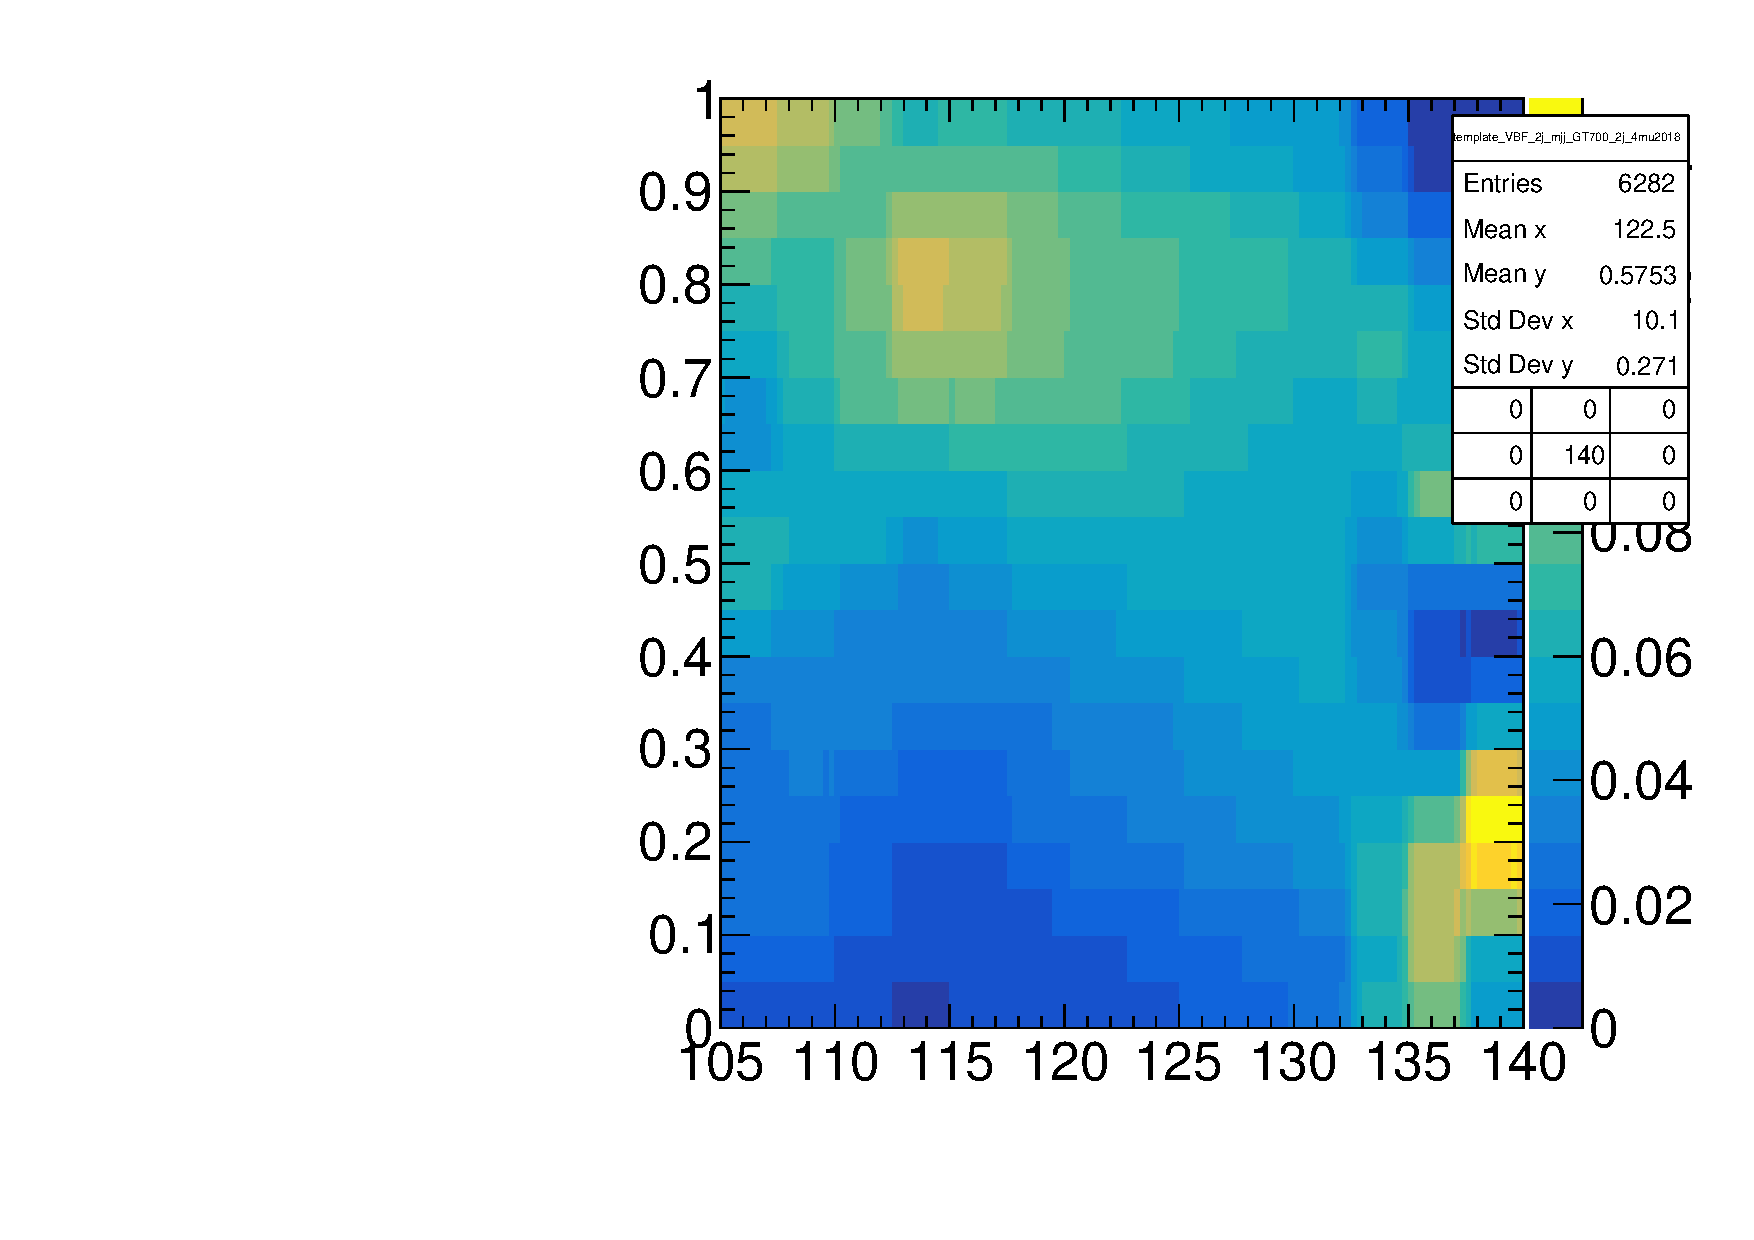
\includegraphics[width=0.45\textwidth]{Figures/Observables/template_VBF_2j_mjj_GT700_2j_4mu2018template.pdf}\\%Observables/Templates_4mu_Untagged_VBFH.pdf} \\
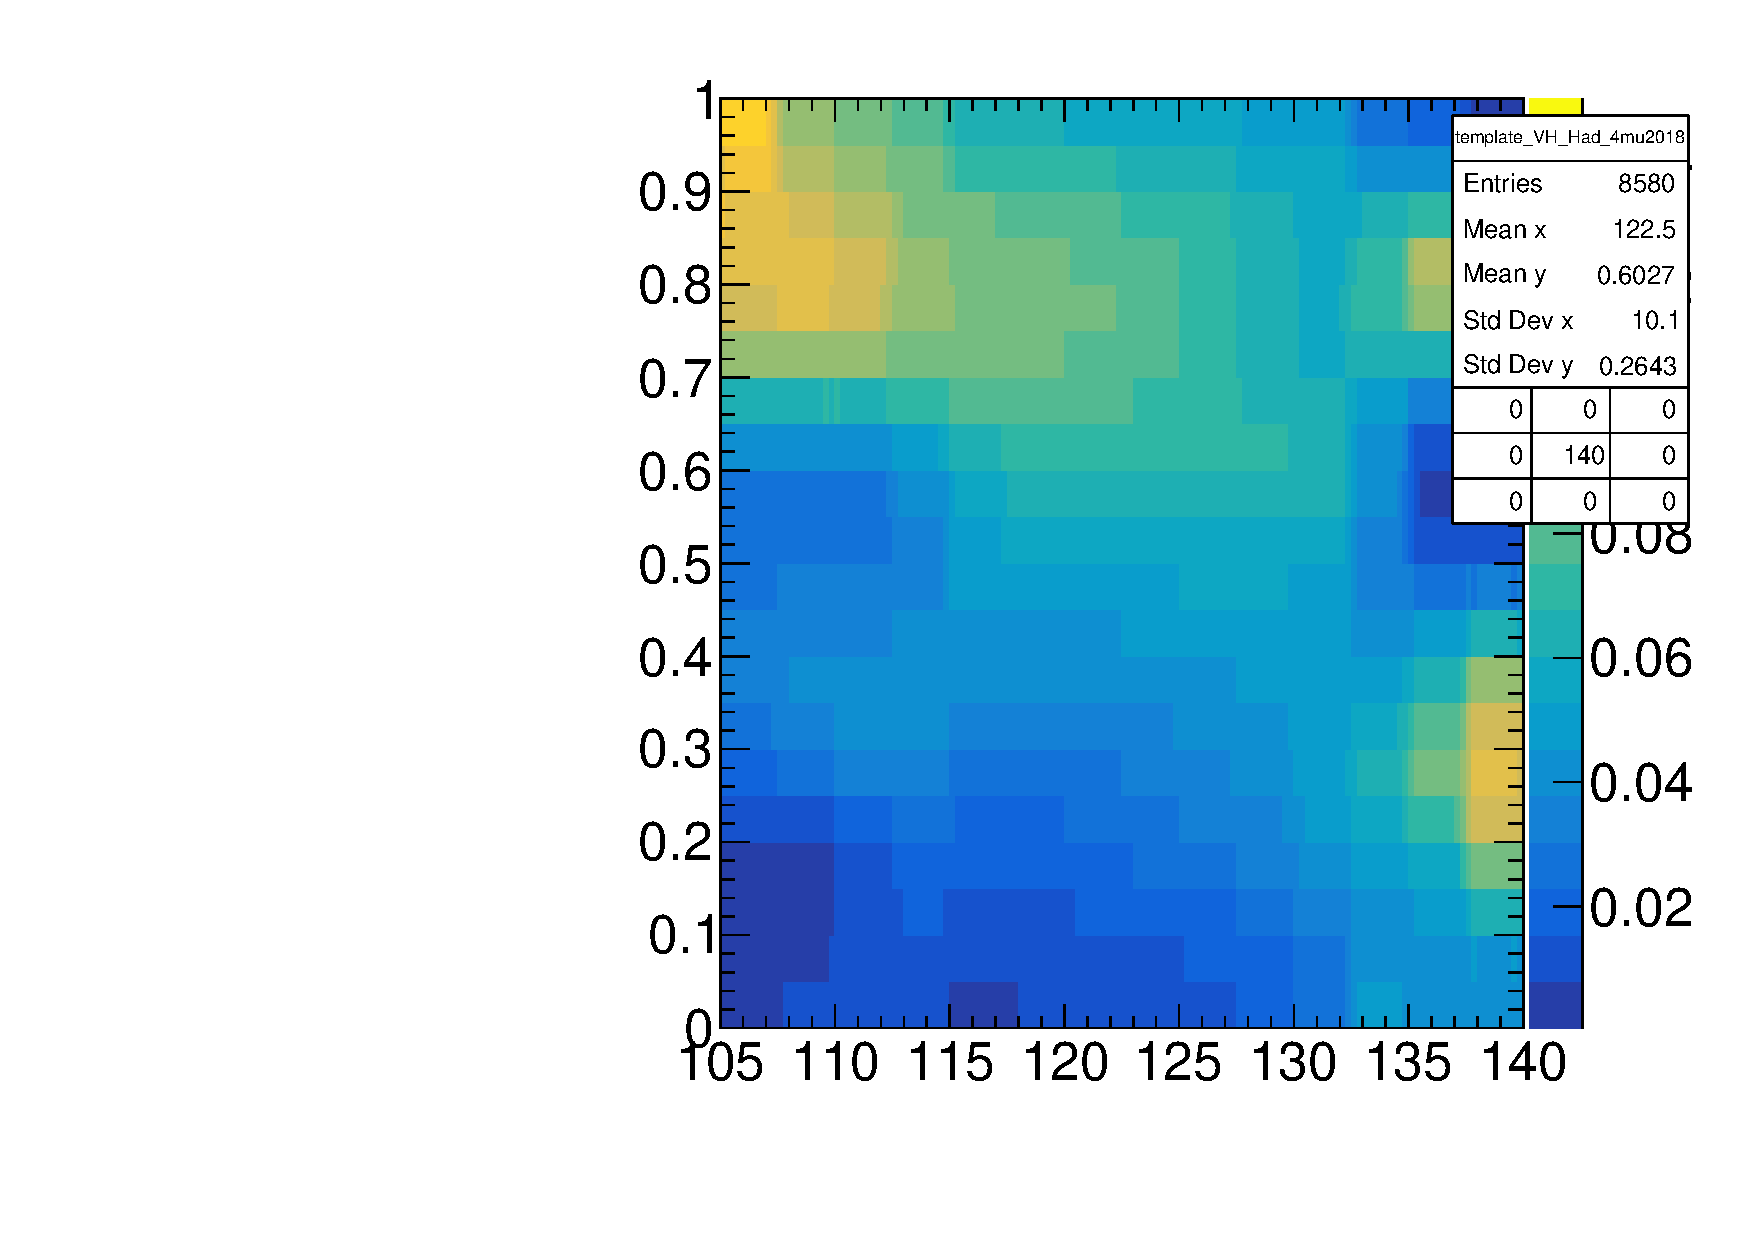
\includegraphics[width=0.45\textwidth]{Figures/Observables/template_VH_Had_4mu2018template.pdf}%Observables/Templates_4mu_Untagged_ZH.pdf}
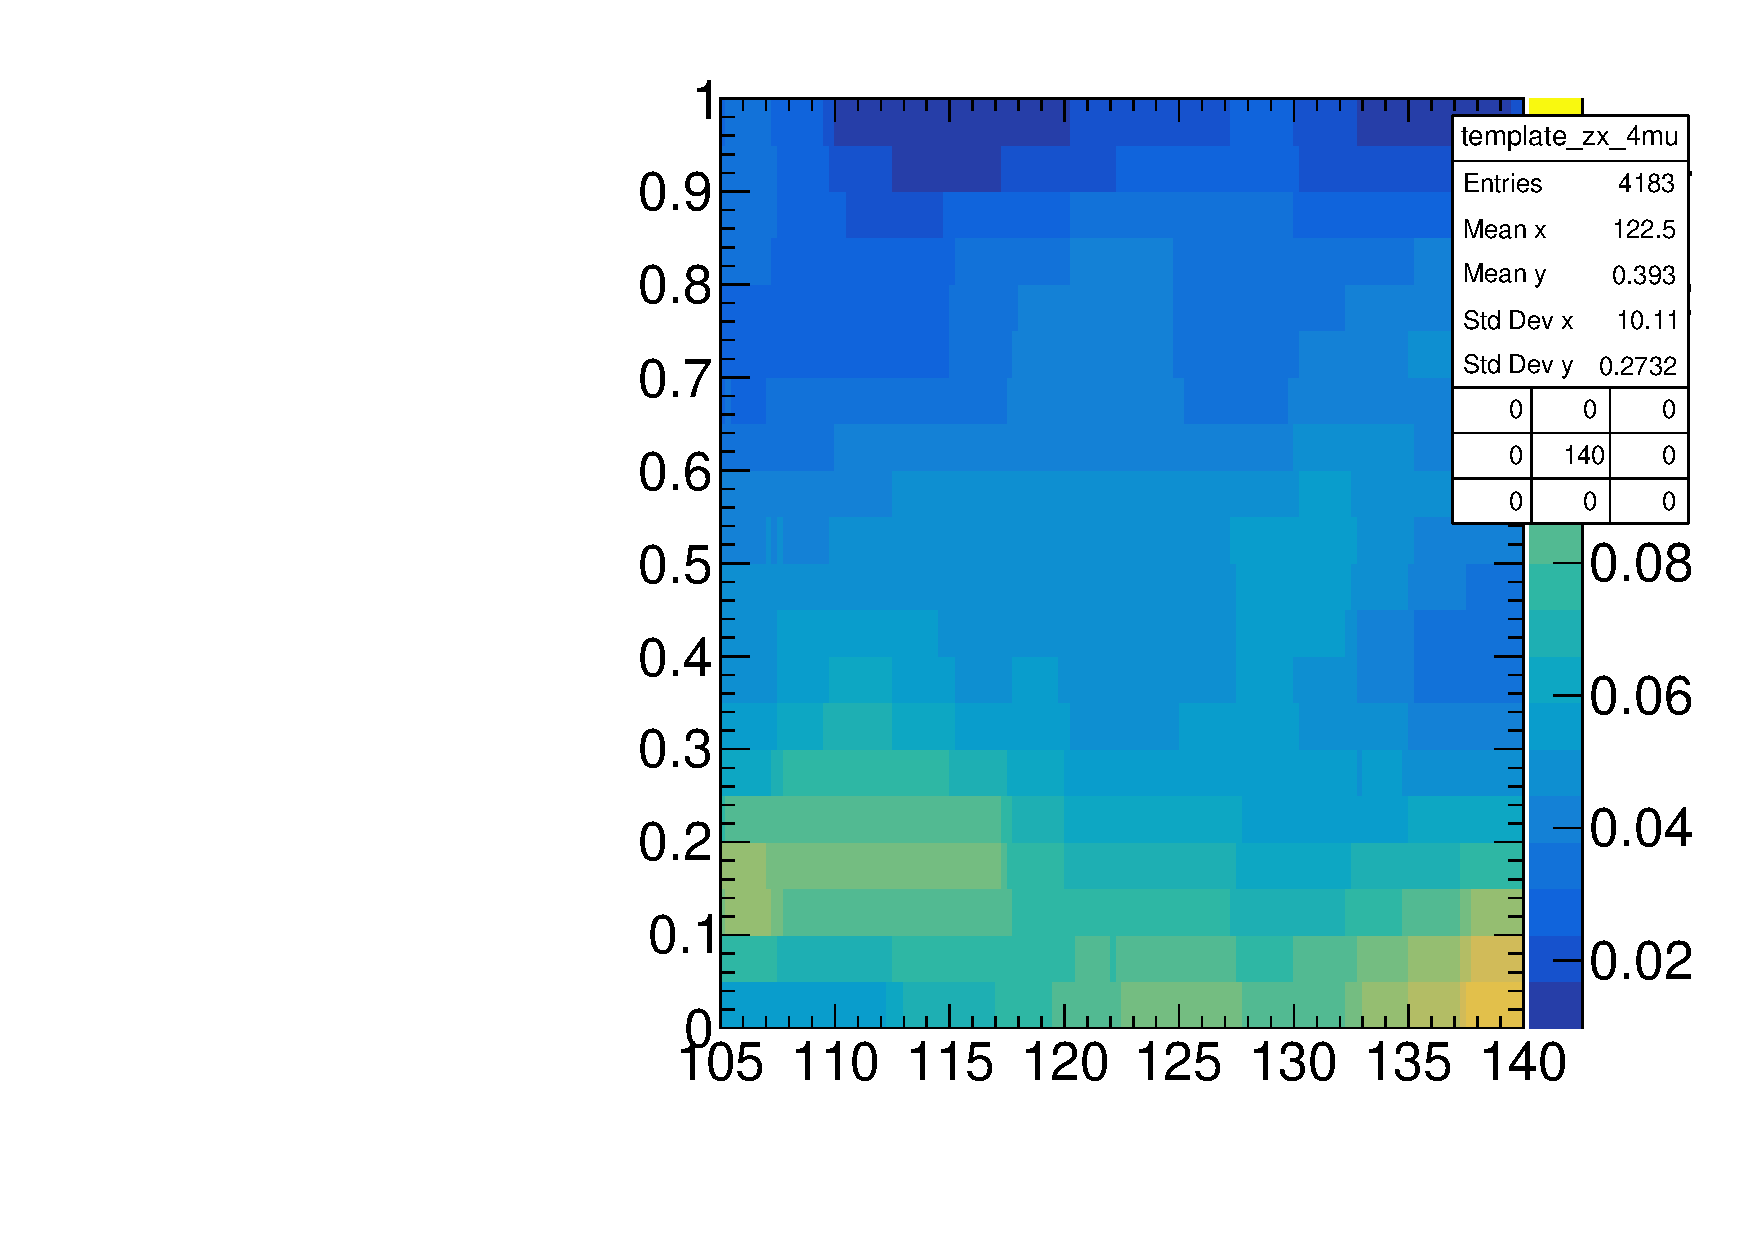
\includegraphics[width=0.45\textwidth]{Figures/Observables/zx_4mu2018template.pdf}\\%Observables/Templates_4mu_Untagged_ZpX.pdf} \\
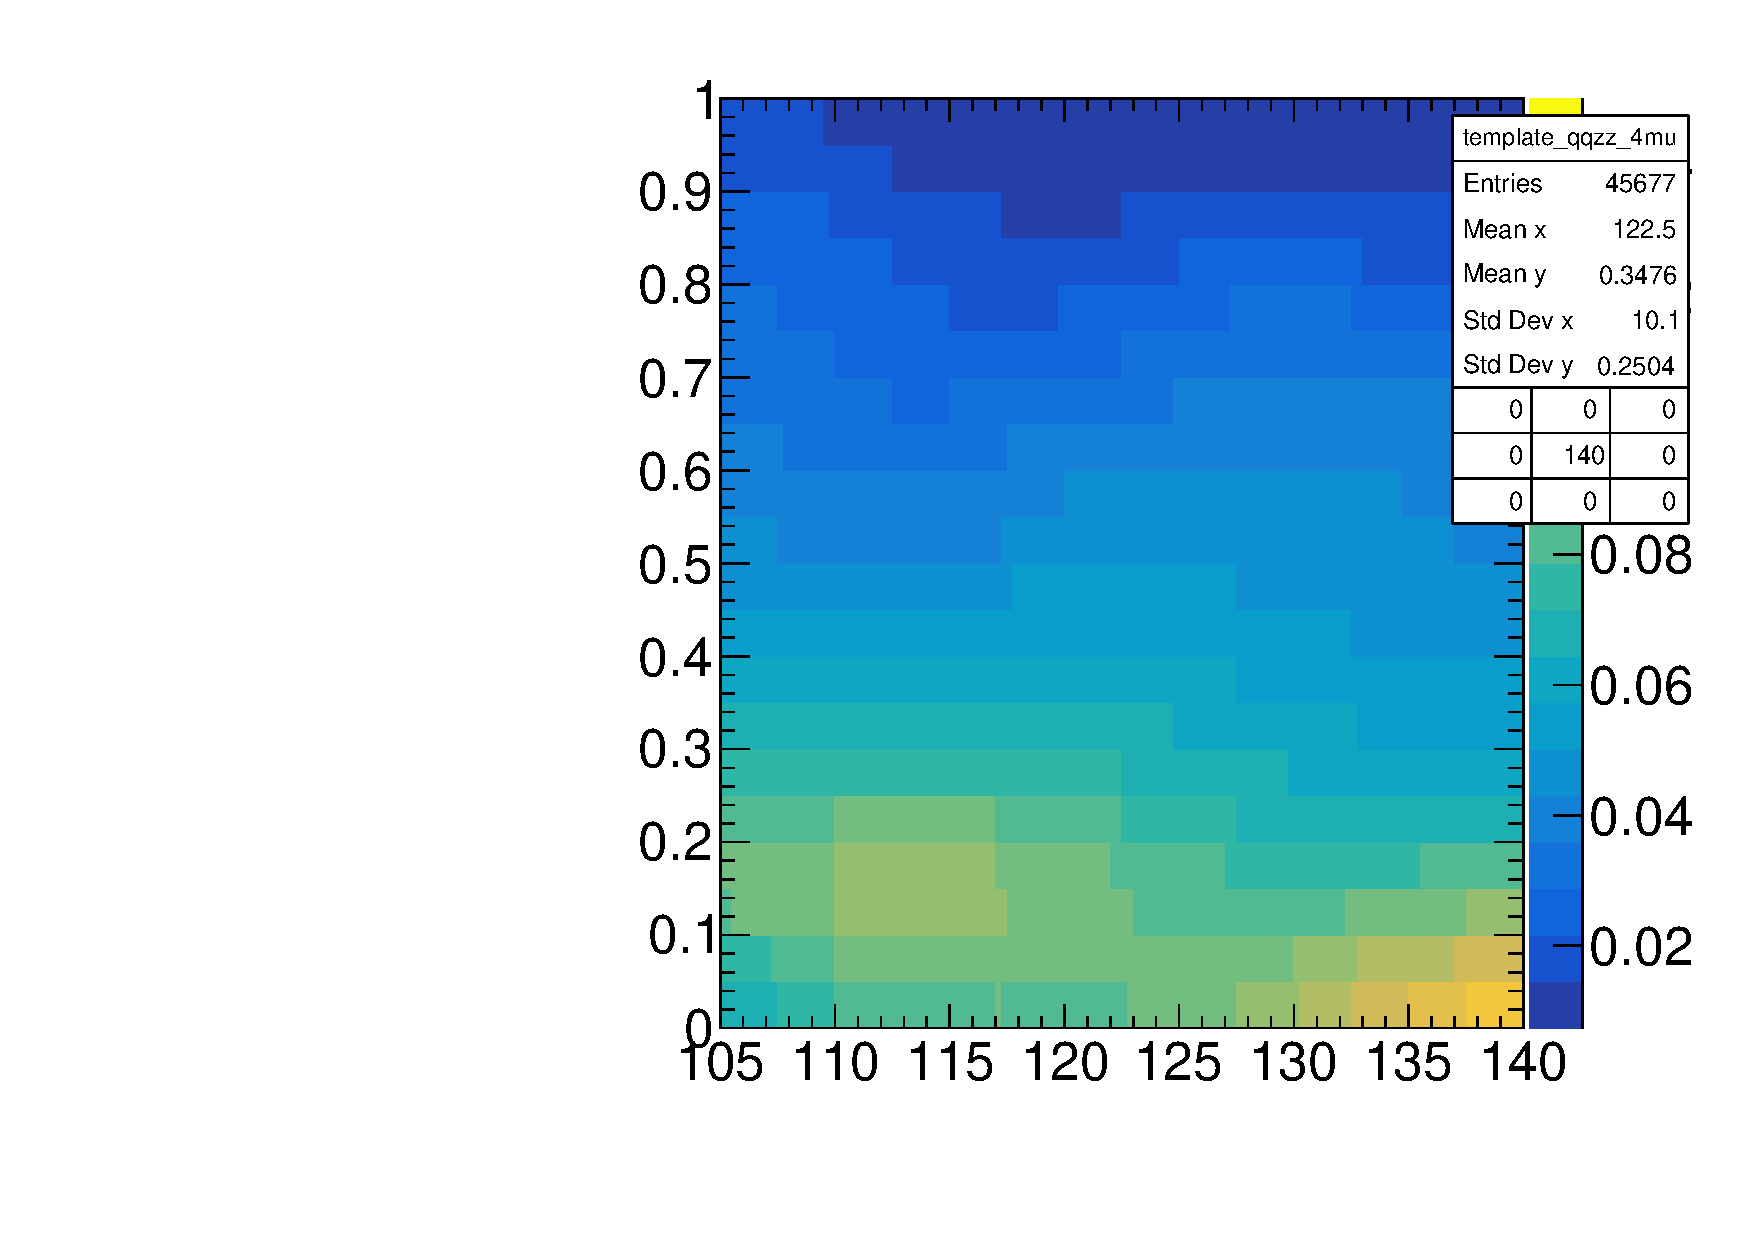
\includegraphics[width=0.45\textwidth]{Figures/Observables/qqzz_4mu2018template.pdf}%Observables/Templates_4mu_Untagged_qqZZ.pdf}
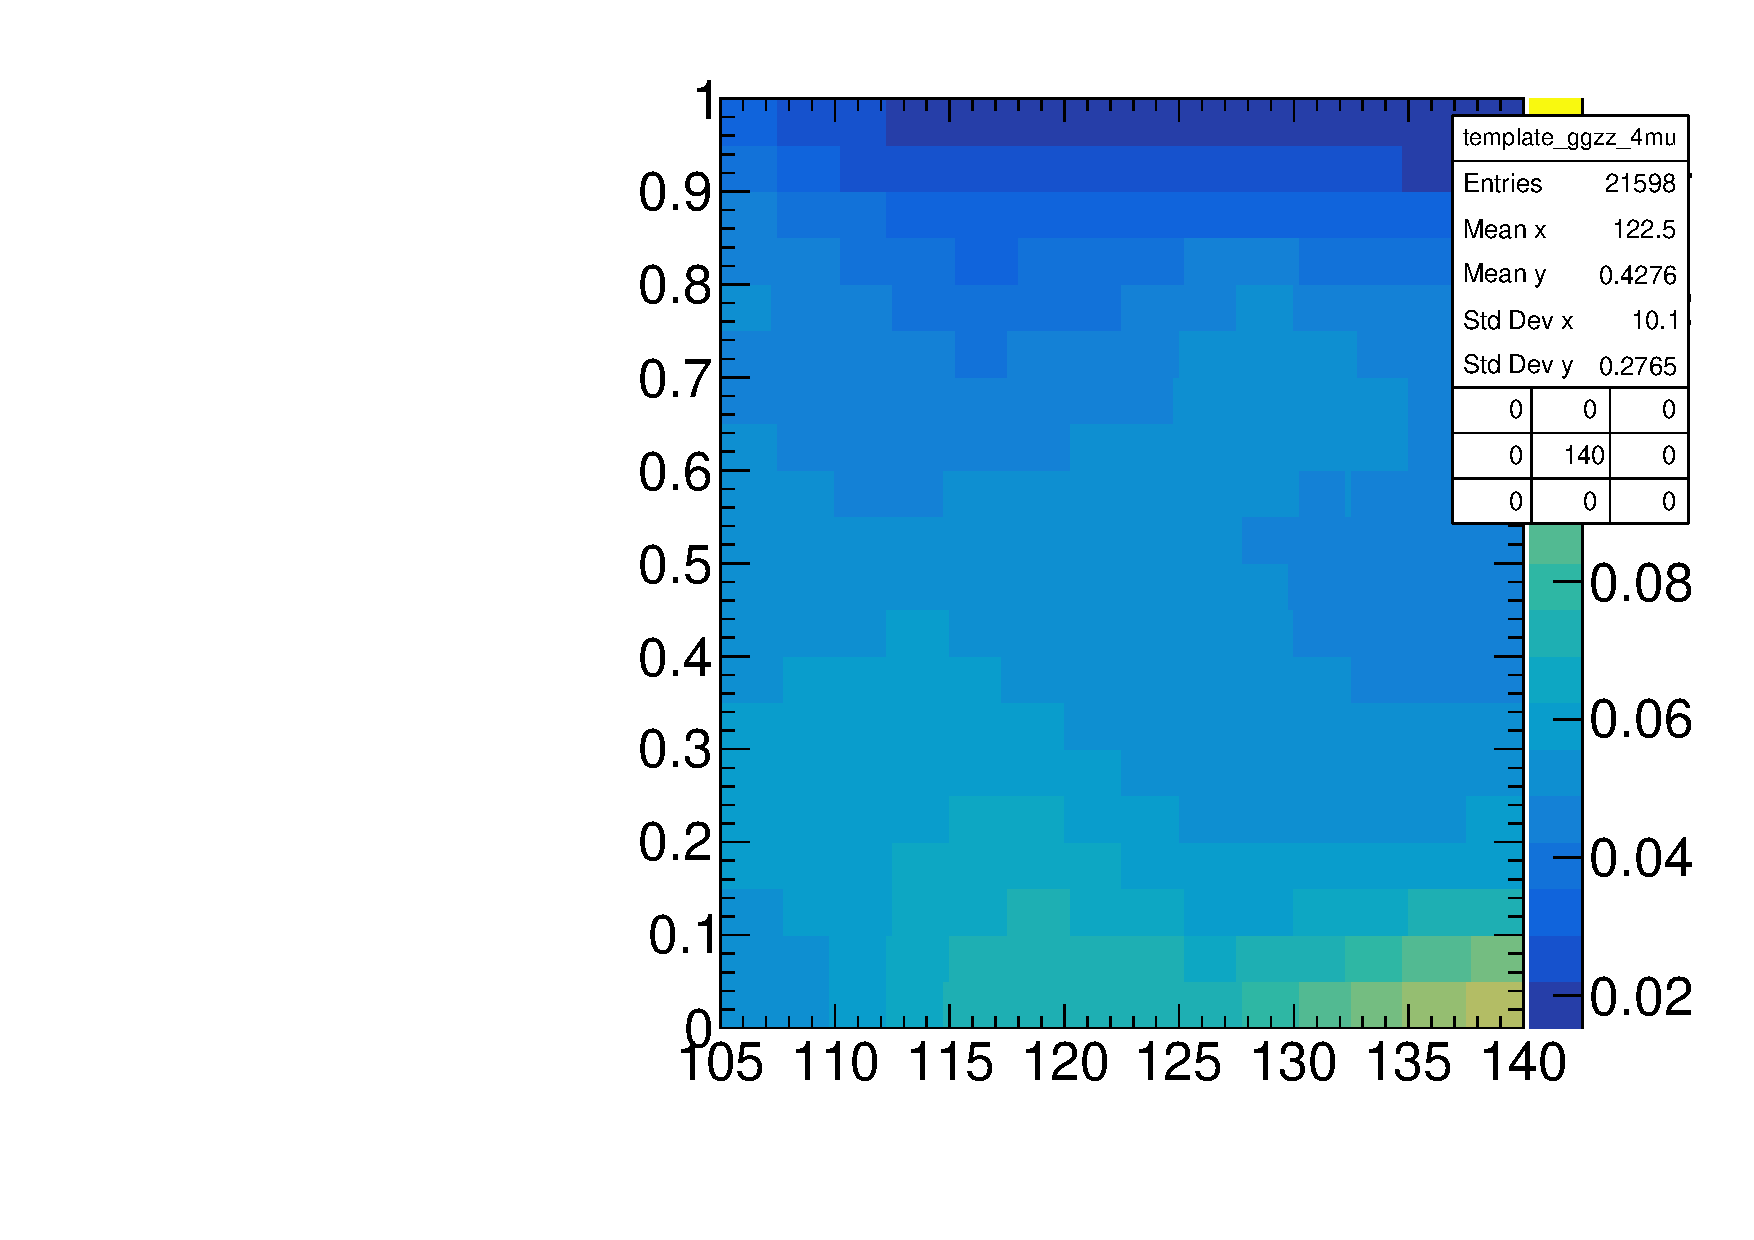
\includegraphics[width=0.45\textwidth]{Figures/Observables/ggzz_4mu2018template.pdf}%Observables/Templates_4mu_Untagged_ggZZ.pdf}
\caption{
Conditional distribution of $\mathcal{D}^{\rm kin}_{\rm bkg}$ in Untagged category for ggH signal (top left), VBF signal (top right), ZH signal (middle left), Z+X background (middle right), $q\bar{q}\to 4\ell$ (bottom left) and $gg\to$ZZ (bottom right) as a function of $m_{4\ell}$.
\label{fig:dbkgkin}}
\end{center}
\end{figure}
%=======

One of the main improvements brought by this analysis is the usage of a new kinematic discriminant. In the final statistical analysis, the signal strength is computed via a 2D fit using the information on the invariant mass of the four leptons and $\mathcal{D}^{\rm kin}_{\rm bkg} $. However, in VBF and VH-hadronic categories, the contamination from ggH process is still important. In order to better separate ggH from the other production modes and from the backgrounds, the idea is thus to add the jet information (i.e., information about the production mode) to the already present information on decay. 

The new dedicated production-dependent $\mathcal{D}_\text{bkg}$ discriminants used in the VBF-2jet tagged and hadronic \VH tagged categories are then defined as:
%%=======
\begin{eqnarray}
\DbkgVBFdec = \frac{\mathcal{P}^{\mathrm{VBF}+\VH+\mathrm{dec}}_\mathrm{sig}(\vec\Omega) }{\mathcal{P}^{\mathrm{VBF}+\VH+\mathrm{dec}}_\mathrm{sig}(\vec\Omega) + c^{\mathrm{VBF 2jet}}(\mell) \times (\mathcal{P}^{\mathrm{VBS}+\VVV}_\mathrm{bkg}(\vec\Omega)+\mathcal{P}^{\mathrm{QCD}+\mathrm{dec}}_\mathrm{bkg}(\vec\Omega)) } \nonumber \\ 
\DbkgVHdec = \frac{\mathcal{P}^{\mathrm{VBF}+\VH+\mathrm{dec}}_\mathrm{sig}(\vec\Omega) }{\mathcal{P}^{\mathrm{VBF}+\VH+\mathrm{dec}}_\mathrm{sig}(\vec\Omega) + c^{\mathrm{had. VH}}(\mell) \times (\mathcal{P}^{\mathrm{VBS}+\VVV}_\mathrm{bkg}(\vec\Omega)+\mathcal{P}^{\mathrm{QCD}+\mathrm{dec}}_\mathrm{bkg}(\vec\Omega)) },
\label{eq:newDbkg} %
\end{eqnarray}
%%=======
where $c^p(\mell)$ for category $p$ is the $\mell$-dependent constant to calibrate the distribution. The performance of the new background discriminants in these categories are compared to \Dbkgkin on Fig.~\ref{fig:rocnewDbkg} as ROC curves.

%%%%%%%%%%%%%%%%%%%%%%%%%%%%%
\begin{figure*}[tbh]
\centering
	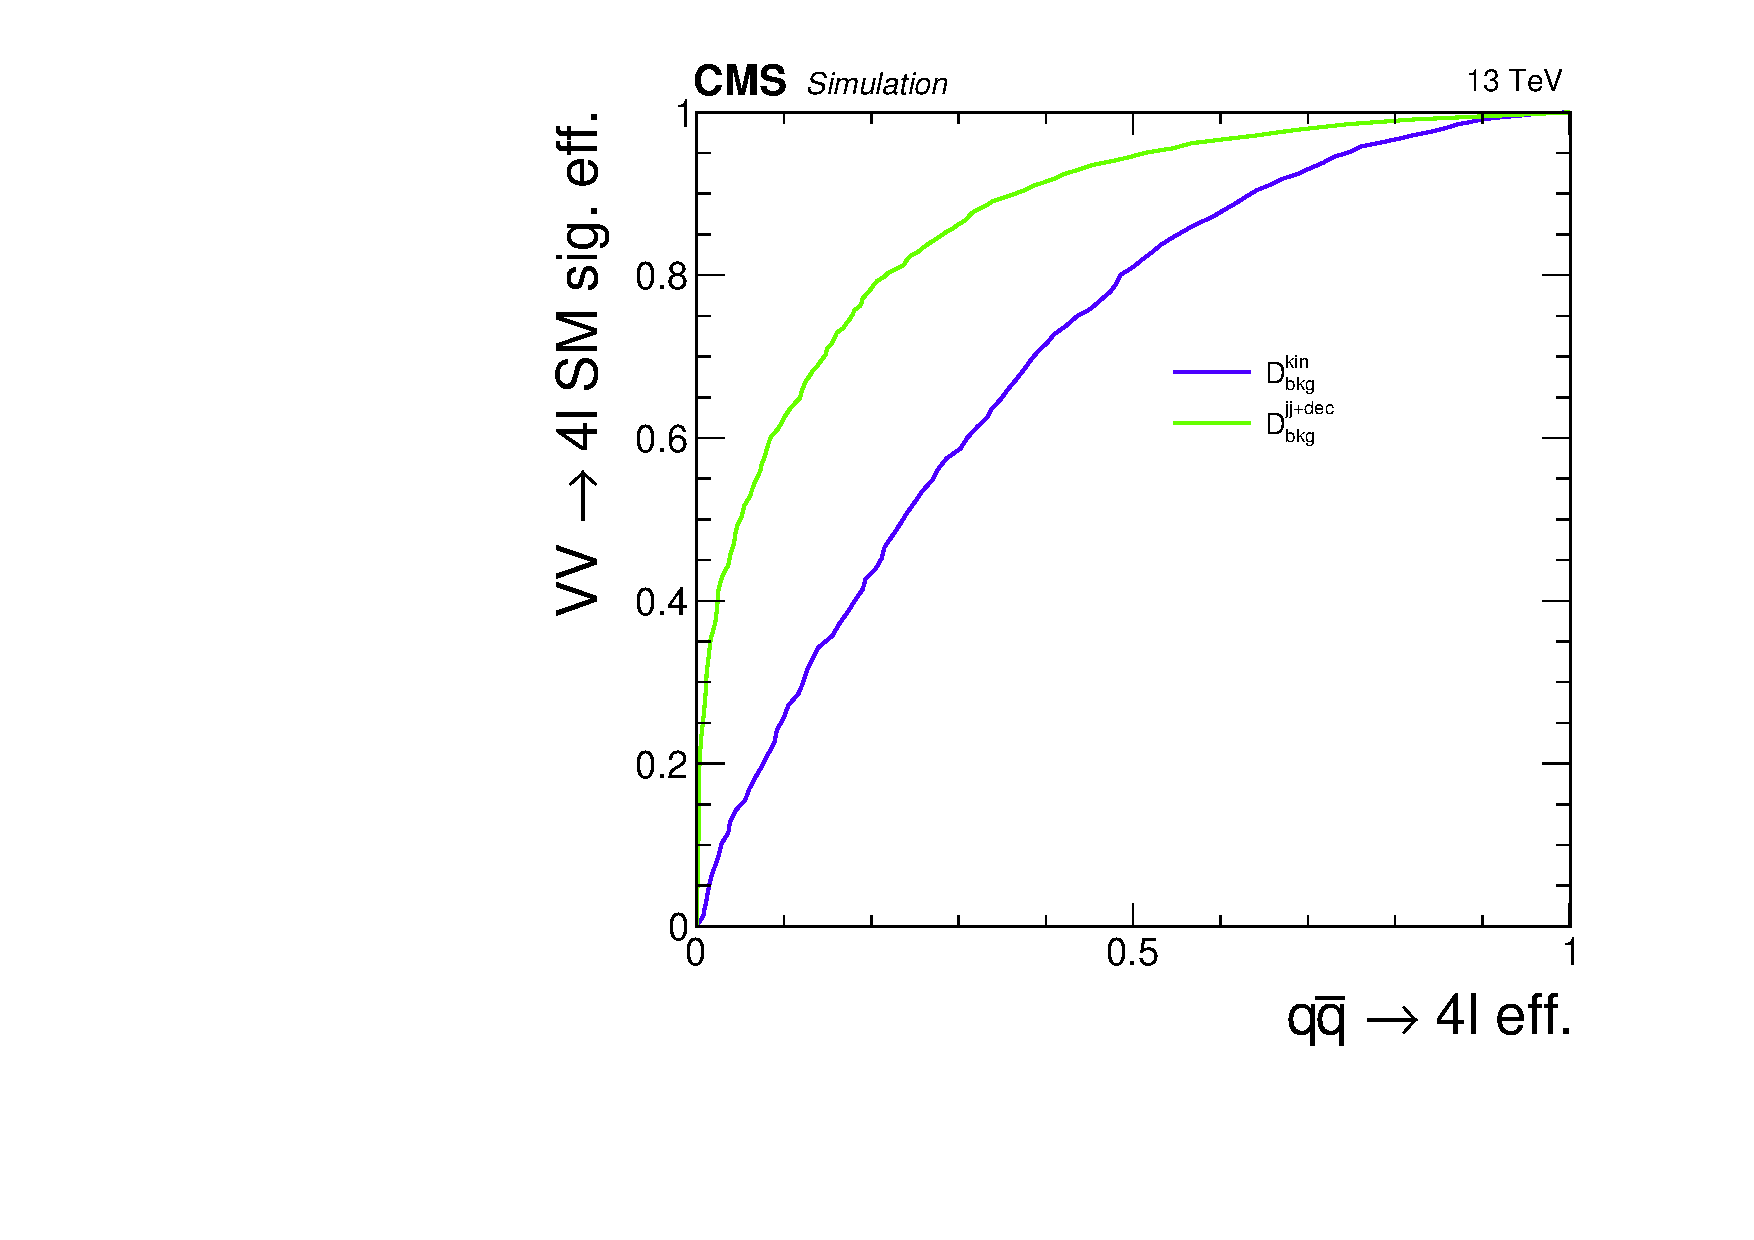
\includegraphics[width=.4\textwidth]{Figures/Observables/ROC_VVZZ_offshell_Sig_vs_qqZZ_2e2mu_JJVBFTagged_ZZMass_105_140.pdf}
	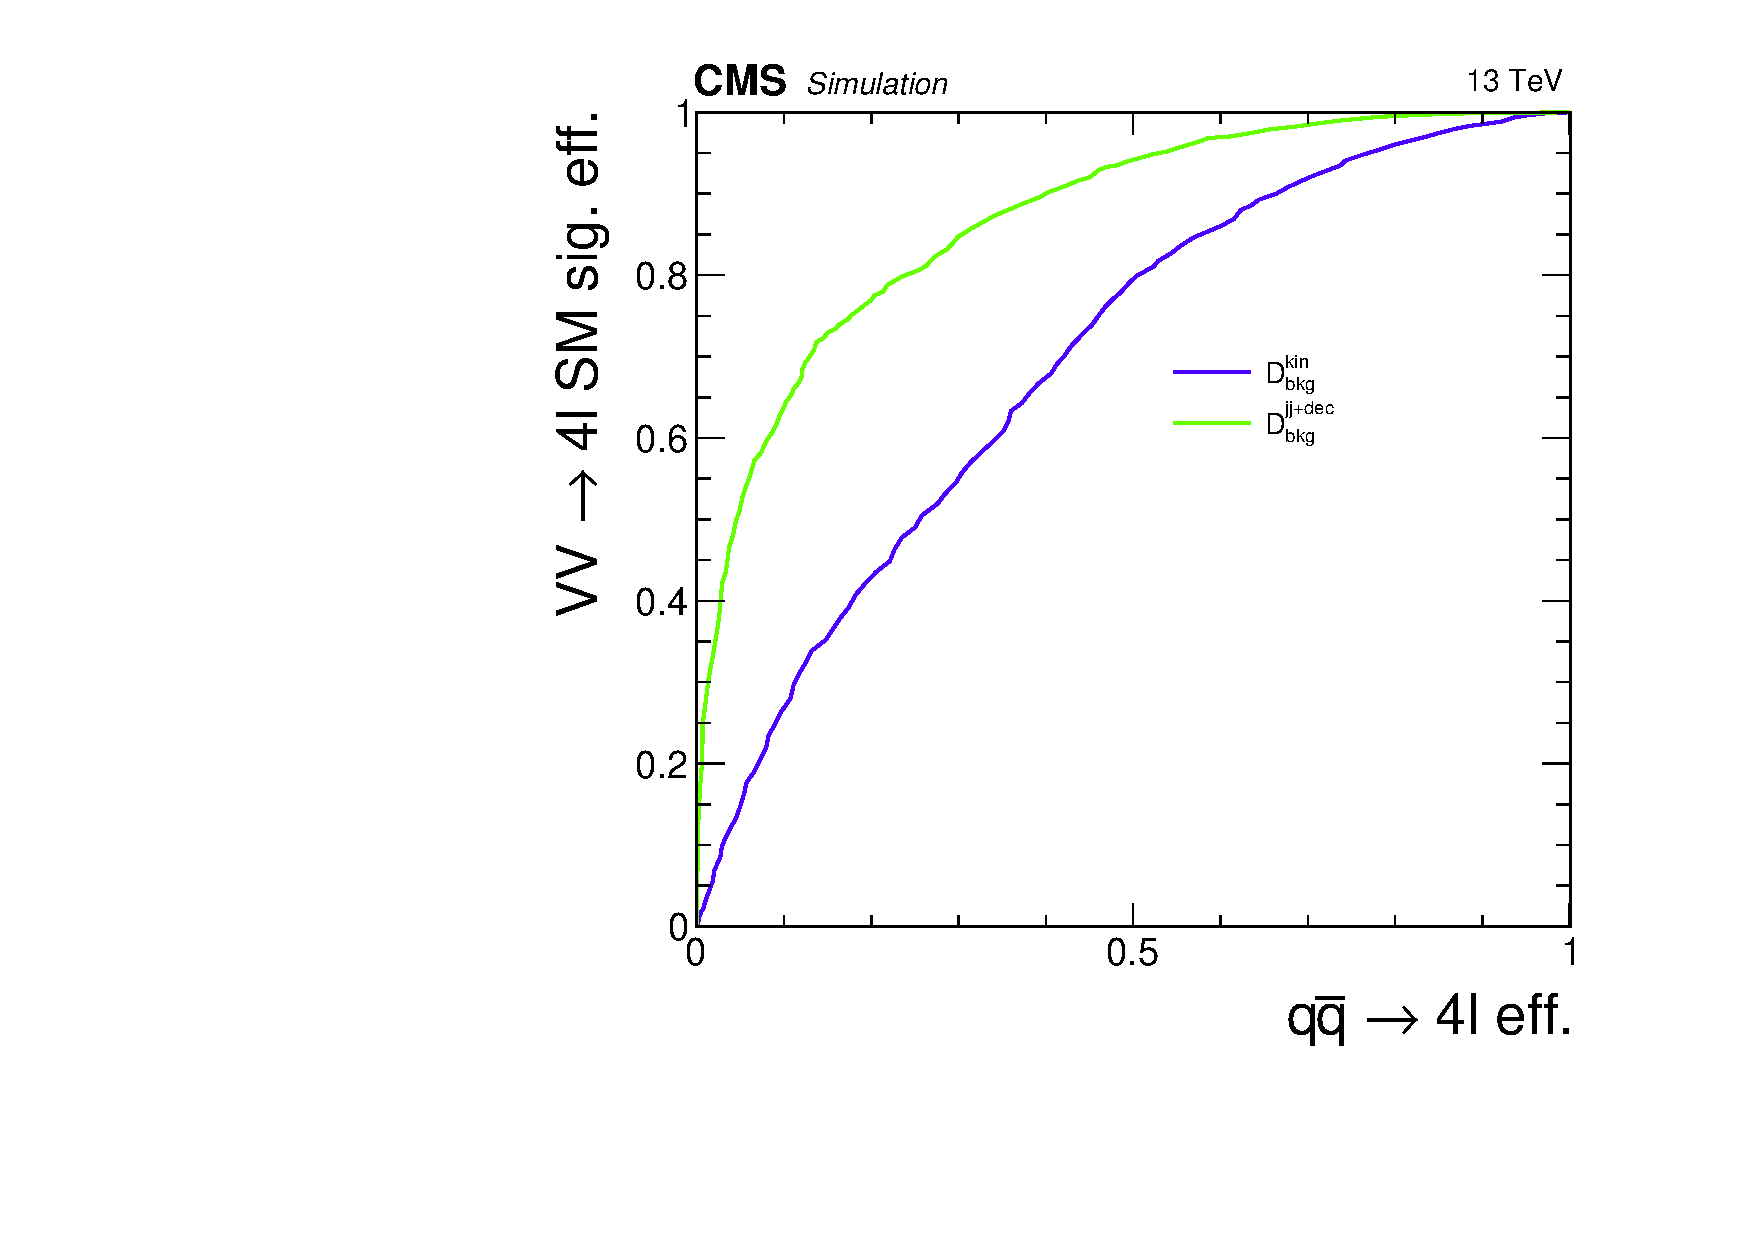
\includegraphics[width=.4\textwidth]{Figures/Observables/ROC_VVZZ_offshell_Sig_vs_qqZZ_2e2mu_HadVHTagged_ZZMass_105_140.pdf}
	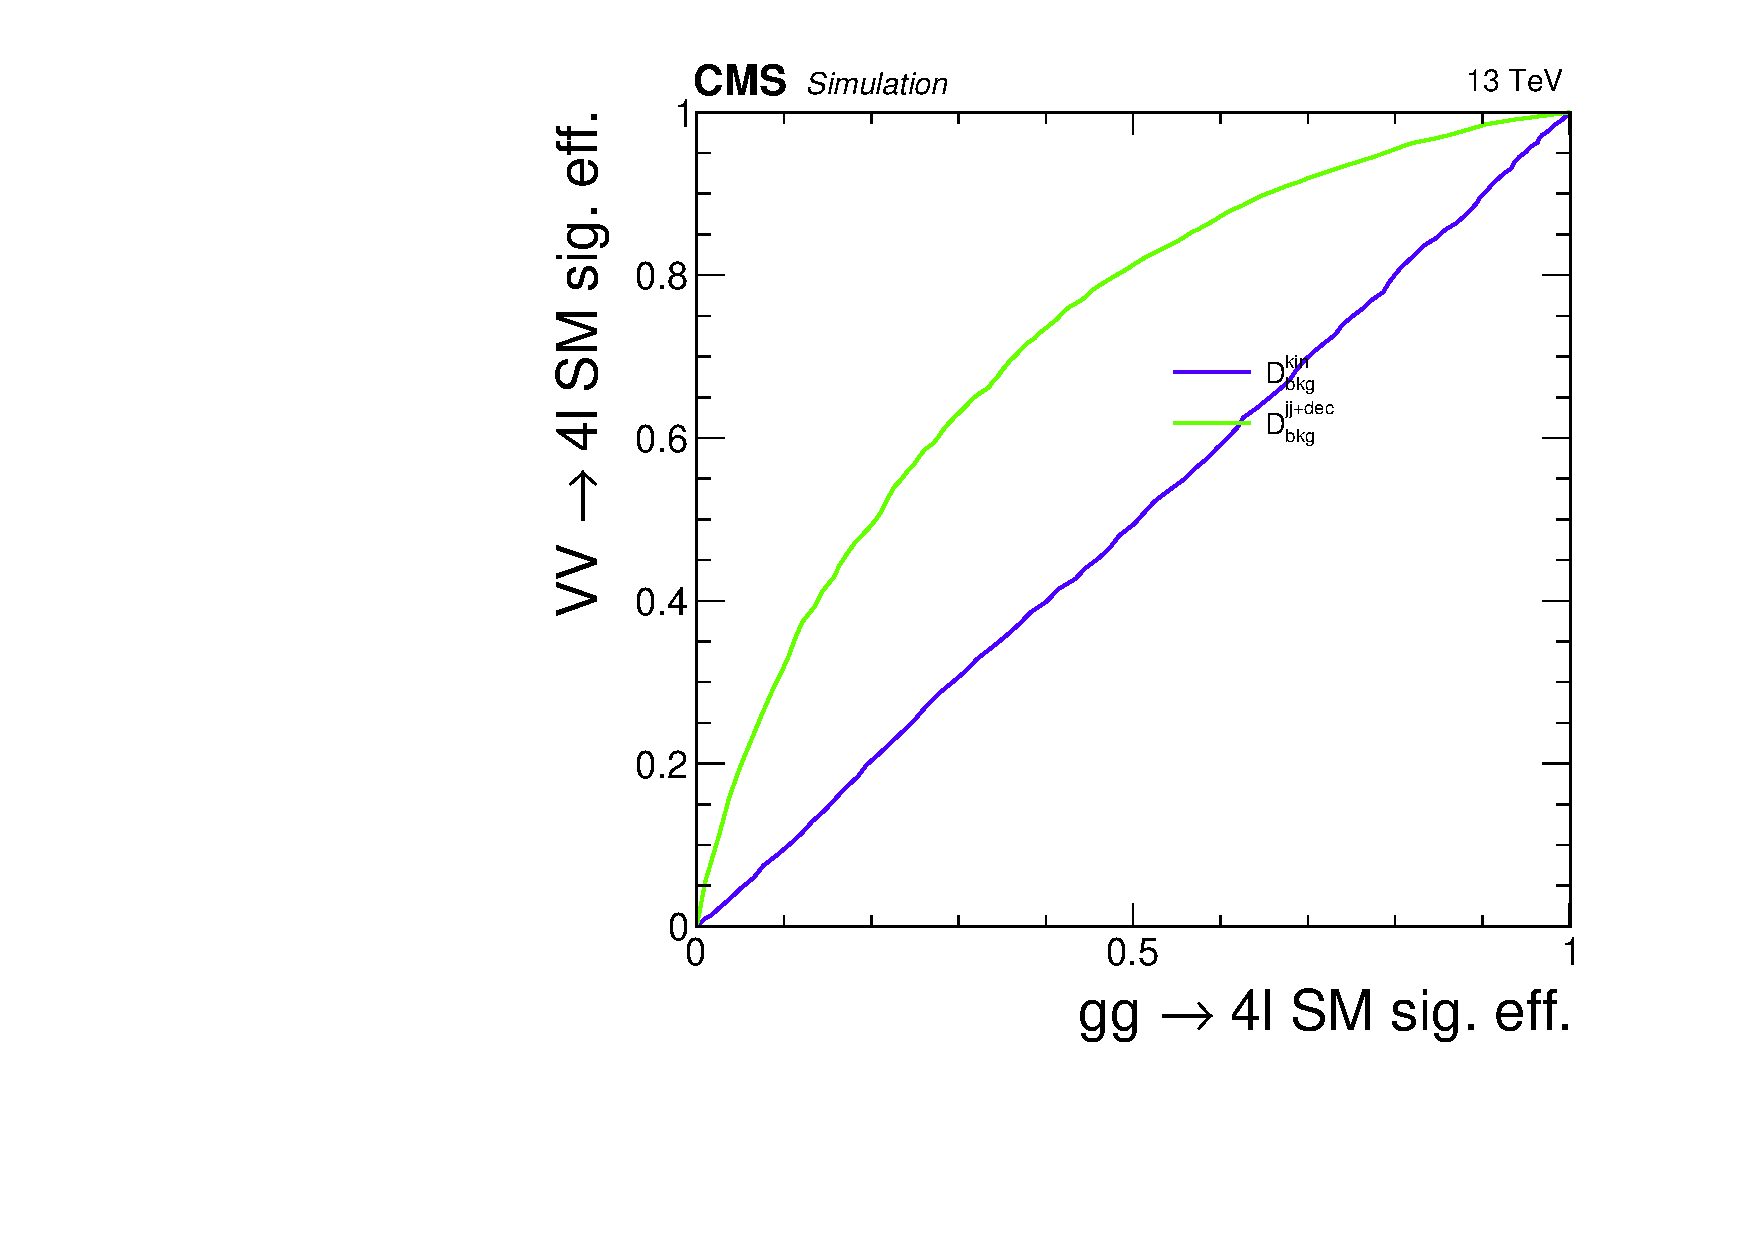
\includegraphics[width=.4\textwidth]{Figures/Observables/ROC_VVZZ_offshell_Sig_vs_ggZZ_offshell_Sig_2e2mu_JJVBFTagged_ZZMass_105_140.pdf}
	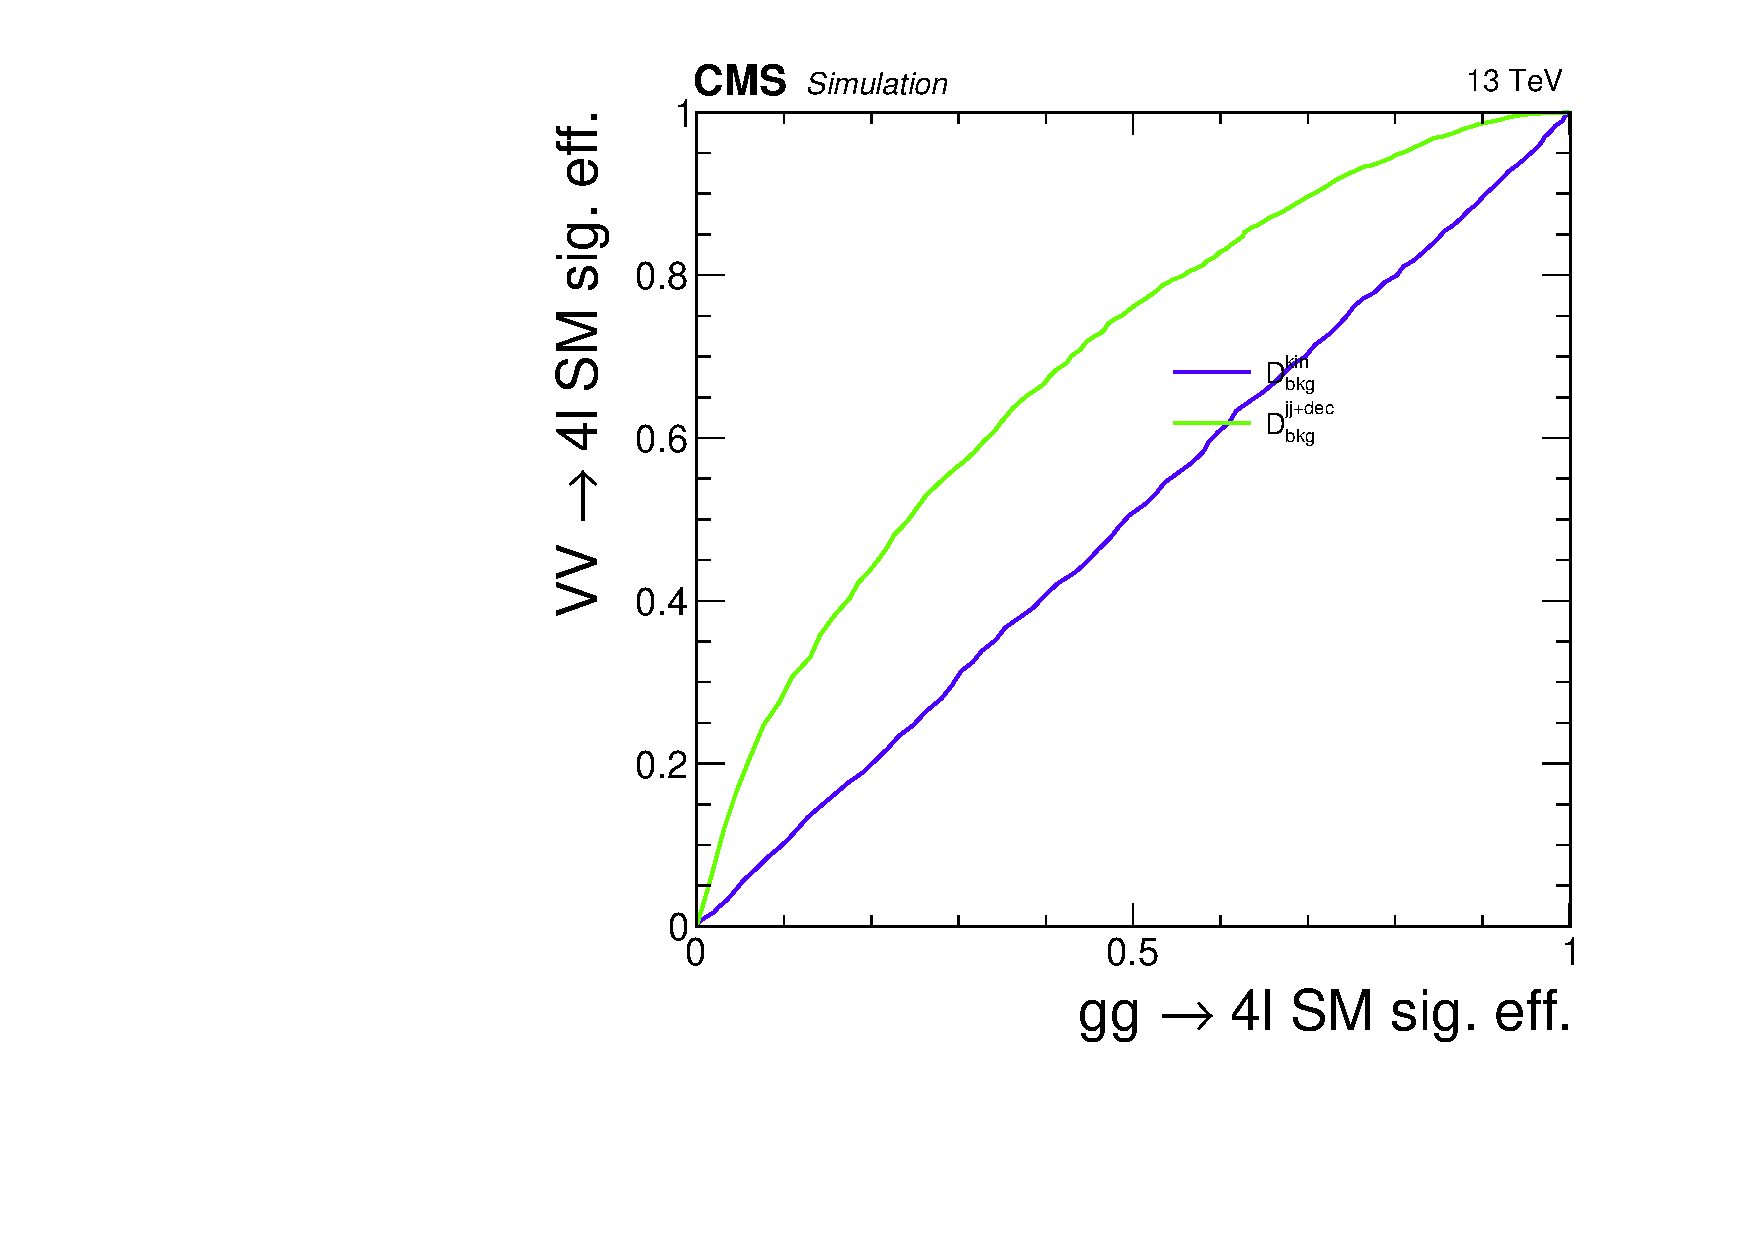
\includegraphics[width=.4\textwidth]{Figures/Observables/ROC_VVZZ_offshell_Sig_vs_ggZZ_offshell_Sig_2e2mu_HadVHTagged_ZZMass_105_140.pdf}
\caption{
Top panels: Comparison of \DbkgVBFdec and \Dbkgkin in the VBF-2jet tagged category (\cmsLeft) and 
\DbkgVHdec and \Dbkgkin in the had. \VH tagged category (\cmsRight) between the VBF (\cmsLeft) or VH (\cmsRight) processes and the \qqbar background. 
Bottom panels: Comparison of \DbkgVBFdec and \Dbkgkin in the VBF-2jet tagged category (\cmsLeft) and 
\DbkgVHdec and \Dbkgkin in the had. \VH tagged category (\cmsRight) between the VBF (\cmsLeft) or VH (\cmsRight) processes and the gluon fusion signal process.
\label{fig:rocnewDbkg}
}
\end{figure*}
%%%%%%%%%%%%%%%%%%%%%%%%%%%%%

A test of this new discriminant was performed, running the full statistical analysis. The likelihood scans for the expected signal strength modifiers corresponding to the five main Higgs production modes were computed for the nominal configuration and for the one using kinematic discriminant with jet information:
\begin{itemize}
\item~$\mu_{VBF}$ went from $+0.999^{+1.224}_{-0.937}$ to  $+0.999^{+1.152}_{-0.783}$
\item~$\mu_{VH-had}$ went from $+0.998^{+3.851}_{-0.998}$ to  $+0.999^{+3.286}_{-0.999}$
\end{itemize}

leading thus to an improvement of about 10 to 15 percent. 

%Figure~\ref{fig:dbkgkinVBF} (resp. Figure~\ref{fig:dbkgkinVH} shows conditional distribution of $\DbkgVBFdec$ (resp. $\DbkgVHdec$) for signal and backgrounds,  as a function of $m_{4\ell}$, in the VBF-2 jets (resp. VH-hadronic) category.
%$\mathcal{D}^{\rm kin}_{\rm bkg}$ for signal and backgrounds, % $q\bar{q}\to 4\ell$ background as a function of $m_{4\ell}$.

%%=======
%\begin{figure}[!htb]
%\vspace*{0.3cm}
%\begin{center}
%
\includegraphics[width=0.45\textwidth]{Figures/Placeholder.png}%Observables/Templates_4mu_VBF2jTagged_ggH.pdf}
%
\includegraphics[width=0.45\textwidth]{Figures/Placeholder.png}\\%Observables/Templates_4mu_VBF2jTagged_VBFH.pdf} \\
%
\includegraphics[width=0.45\textwidth]{Figures/Placeholder.png}%Observables/Templates_4mu_VBF2jTagged_ZH.pdf}
%
\includegraphics[width=0.45\textwidth]{Figures/Placeholder.png}\\%Observables/Templates_4mu_VBF2jTagged_ZpX.pdf} \\
%
\includegraphics[width=0.45\textwidth]{Figures/Placeholder.png}%Observables/Templates_4mu_VBF2jTagged_qqZZ.pdf}
%
\includegraphics[width=0.45\textwidth]{Figures/Placeholder.png}%Observables/Templates_4mu_VBF2jTagged_ggZZ.pdf}
%\caption{
%Conditional distribution of $\mathcal{D}^{\rm kin}_{\rm bkg}$ in VBF-2jets tagged category for ggH signal (top left), VBF signal (top right), ZH signal (middle left), Z+X background (middle right), $q\bar{q}\to 4\ell$ (bottom left) and $gg\to$ZZ (bottom right) as a function of $m_{4\ell}$.
%\label{fig:dbkgkinVBF}}
%\end{center}
%\end{figure}
%%=======
%
%%=======
%\begin{figure}[!htb]
%\vspace*{0.3cm}
%\begin{center}
%
\includegraphics[width=0.45\textwidth]{Figures/Placeholder.png}%Observables/Templates_4mu_VHHadrTagged_ggH.pdf}
%
\includegraphics[width=0.45\textwidth]{Figures/Placeholder.png}\\%Observables/Templates_4mu_VHHadrTagged_VBFH.pdf} \\
%
\includegraphics[width=0.45\textwidth]{Figures/Placeholder.png}%Observables/Templates_4mu_VHHadrTagged_ZH.pdf}
%
\includegraphics[width=0.45\textwidth]{Figures/Placeholder.png}\\%Observables/Templates_4mu_VHHadrTagged_ZpX.pdf} \\
%
\includegraphics[width=0.45\textwidth]{Figures/Placeholder.png}%Observables/Templates_4mu_VHHadrTagged_qqZZ.pdf}
%
\includegraphics[width=0.45\textwidth]{Figures/Placeholder.png}%Observables/Templates_4mu_VHHadrTagged_ggZZ.pdf}
%\caption{
%Conditional distribution of $\mathcal{D}^{\rm kin}_{\rm bkg}$ in VH-hadronic tagged category for ggH signal (top left), VBF signal (top right), ZH signal (middle left), Z+X background (middle right), $q\bar{q}\to 4\ell$ (bottom left) and $gg\to$ZZ (bottom right) as a function of $m_{4\ell}$.
%\label{fig:dbkgkinVH}}
%\end{center}
%\end{figure}
%%=======

%Figure~\ref{fig:melavsmass} shows conditional templates of $\mathcal{D}^{\rm kin}_{\rm bkg} $ discriminant 
%for a wide range of $m_{4\ell}$ values, as used in analysis. 
%=============                                                                                                                                     
%\begin{figure}[!htb]
%\vspace*{0.3cm}
%\begin{center}
%
\includegraphics[width=0.45\textwidth]{Figures/Placeholder.png}
%
\includegraphics[width=0.45\textwidth]{Figures/Placeholder.png}
%
\includegraphics[width=0.45\textwidth]{Figures/Placeholder.png}
%
\includegraphics[width=0.45\textwidth]{Figures/Placeholder.png}
%\caption
%{
%Distribution of the $\mathcal{D}^{\rm kin}_{\rm bkg} $ discriminant vs $m_{4\ell}$ for
%$H\to ZZ\to 2e2\mu$ signal (top) and $q\bar{q}\to 2e2\mu$ background (bottom)
%in the low-mass (left) and full (right) range of $m_{4\ell}$.
%MC simulation at 13 TeV is shown.
%\label{fig:melavsmass}
%}
%\end{center}
%\end{figure}
%=============                                                                 
                                                                
                                                                                                        
\subsubsection{Kinematic discriminants for categorization}

The discriminant sensitive to the VBF signal topology with two associated jets
is calculated as~\cite{Khachatryan:2015cwa, Khachatryan:2015mma} 
%%%%%%%%%%%%%%%%%%%%%
\begin{eqnarray}
%
\label{eq:vbfmela}
\DMeVbfjj = 
\left[1+
\frac{ \mathcal{P}_{\rm HJJ} (\vec\Omega^{\rm \PH+JJ} | m_{4\ell}) }
{\mathcal{P}_{\rm VBF}  (\vec\Omega^{\rm \PH+JJ} | m_{4\ell})  }\right]^{-1}
\,,
%
\end{eqnarray}
%%%%%%%%%%%%%%%%%%%%%
where $\mathcal{P}_{\rm VBF}$ and $\mathcal{P}_{\rm \PH JJ}$ are probabilities obtained from the 
\textsc{JHUGen} matrix elements for the VBF process and gluon fusion (technically combination of
$gg/qg/qq^\prime$ parton collisions)
in association with two jets ($\PH+2$\,jets) within the MELA framework.
This discriminant is equally efficient in separating VBF from either $\Pg\Pg\to\PH+2$\,jets signal or $\Pg\Pg$ 
or $q\bar{q}\to 4\ell+2$\,jets background because jet correlations in these processes are distinct from the VBF process. 

The discriminant sensitive to the VBF signal topology with one associated jet
is calculated as~\cite{Khachatryan:2015cwa, Khachatryan:2015mma} 
%%%%%%%%%%%%%%%%%%%%%
\begin{eqnarray}
%
\label{eq:mela1jet}
\DMeVbfj = 
\left[1+
\frac{ \mathcal{P}_{\rm HJ} (\vec\Omega^{\rm \PH+J} | m_{4\ell}) }
{\int d\eta_{\rm J}\mathcal{P}_{\rm VBF}  (\vec\Omega^{\rm \PH+JJ} | m_{4\ell})  }\right]^{-1}
\,,
%
\end{eqnarray}
%%%%%%%%%%%%%%%%%%%%%
where and $\mathcal{P}_{\rm \PH J}$ is the probability obtained from the 
\textsc{JHUGen} matrix element for gluon fusion in association with one jet ($\PH+1$\,jet) within the 
MELA framework.
The $\int d\eta_{\rm J}\mathcal{P}_{\rm VBF}$ is the integral of the two-jet VBF matrix element probability
discussed above over the $\eta_J$ values of the unobserved jet with the constraint that the total 
transverse momentum of the $HJJ$ system is zero. 

The discriminant sensitive to the VH signal topology with two associated jets 
is calculated as~\cite{Khachatryan:2015cwa, Khachatryan:2015mma} 
%%%%%%%%%%%%%%%%%%%%%
\begin{eqnarray}
%
\label{eq:zhmela}
\DMeWh = 
\left[1+
\frac{ \mathcal{P}_{\rm HJJ} (\vec\Omega^{\rm \PH+JJ} | m_{4\ell}) }
{\mathcal{P}_{\rm ZH}  (\vec\Omega^{\rm \PH+JJ} | m_{4\ell})  }\right]^{-1}
\,, \\
\label{eq:whmela}
\DMeZh = 
\left[1+
\frac{ \mathcal{P}_{\rm HJJ} (\vec\Omega^{\rm \PH+JJ} | m_{4\ell}) }
{\mathcal{P}_{\rm WH}  (\vec\Omega^{\rm \PH+JJ} | m_{4\ell})  }\right]^{-1}
\,, 
%
\end{eqnarray}
%%%%%%%%%%%%%%%%%%%%%
where $\mathcal{P}_{\rm VH}$ and $\mathcal{P}_{\rm \PH JJ}$ are probabilities obtained from the 
\textsc{JHUGen} matrix elements for the VH (either ZH or WH) process and gluon fusion 
in association with two jets ($\PH+2$\,jets) within the MELA framework.

Figure~\ref{fig:melaVBFVH} shows distributions of the four production discriminants discussed above.
In addition, it is possible to calculate ttH, bbH, and tqH discriminants to isolate these production 
mechanisms, using kinematics shown in the last graph of Fig.~\ref{fig:decay}, but expected yields 
in these categories are very small. Therefore full reconstruction needed for the matrix element 
calculation and it will be inefficient with the presently expected statistics. However, for details of such 
matrix element calculations and possible future applications, see Refs.~\cite{AN-16-185,Gritsan:2016hjl}.

%=============                                                                                                                                     
\begin{figure}[!htb]
\vspace*{0.3cm}
\begin{center}
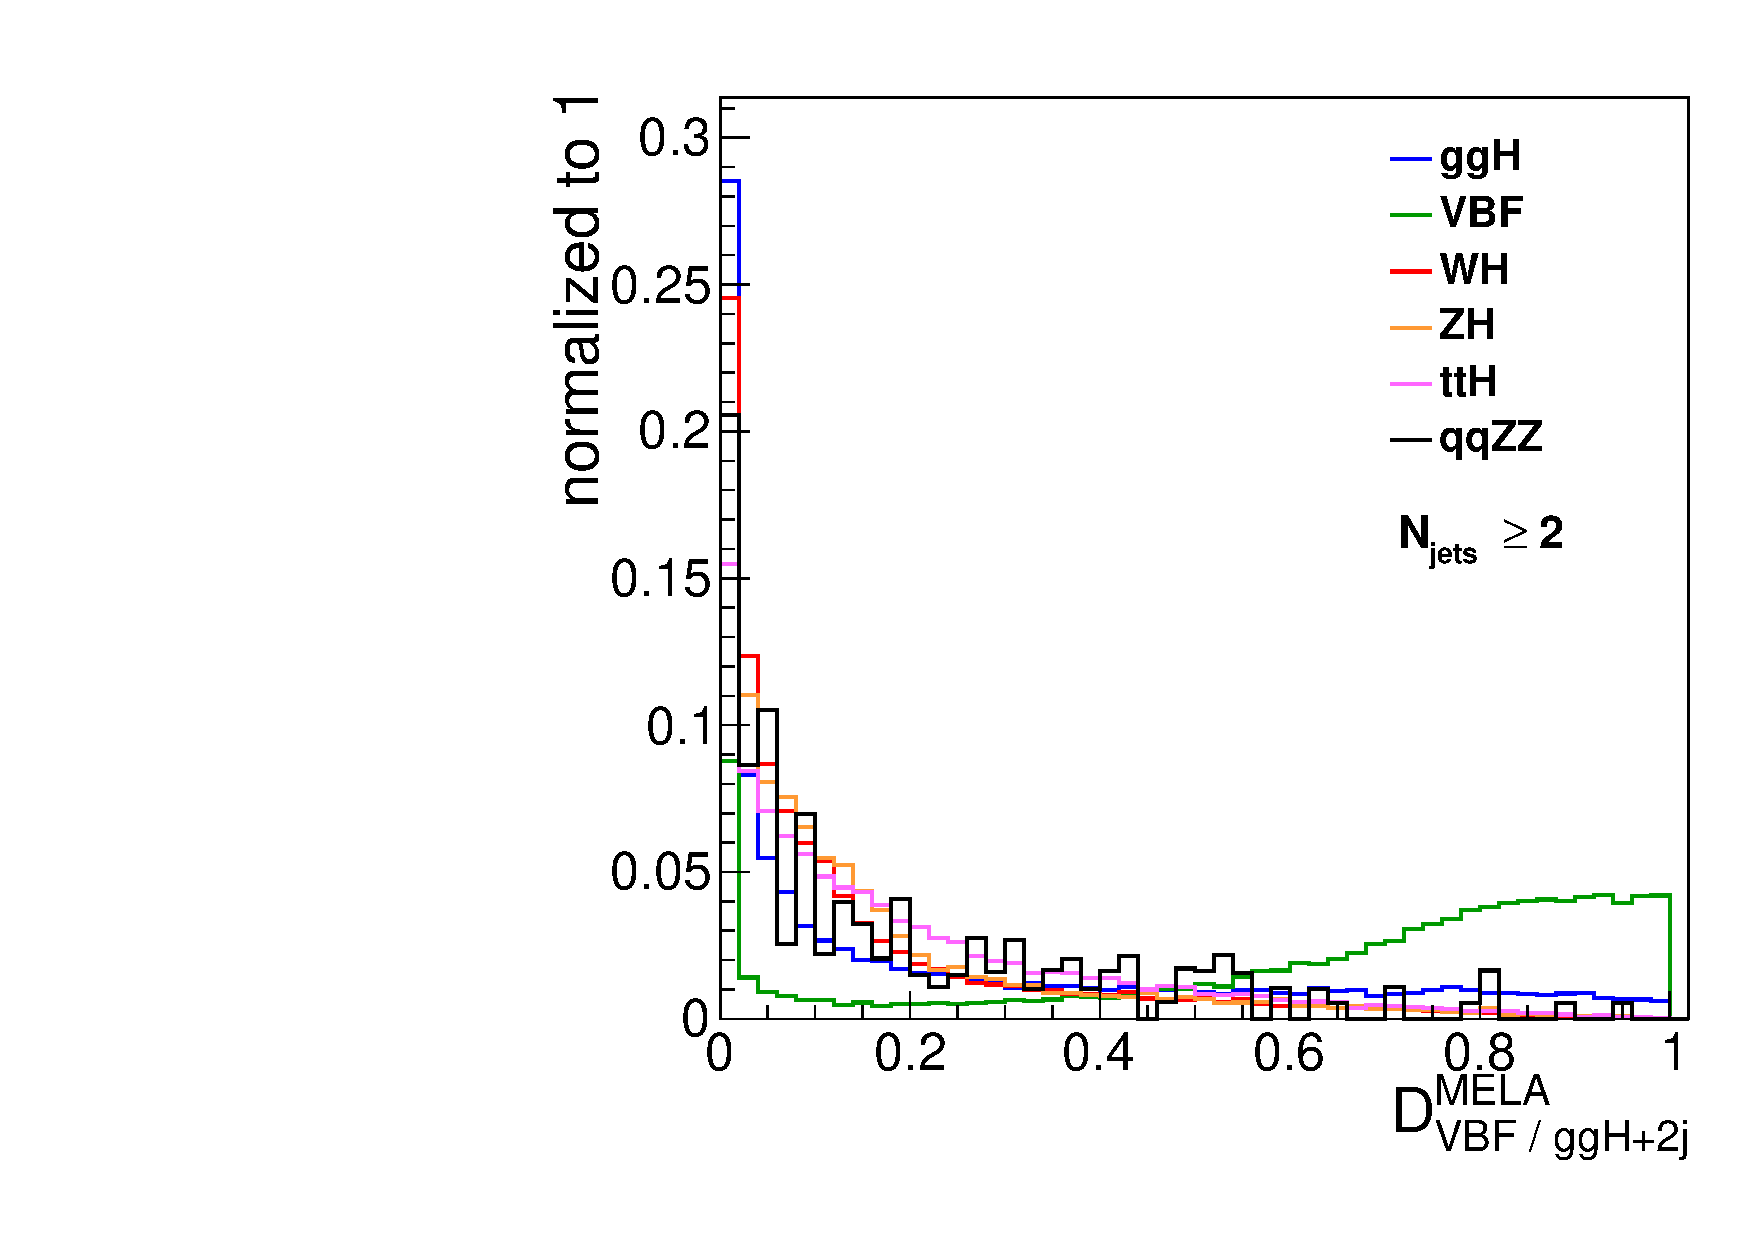
\includegraphics[width=0.45\textwidth]{Figures/Observables/cBCInSR_D2jVbfHjj_m4l118to130_bList10_.pdf}
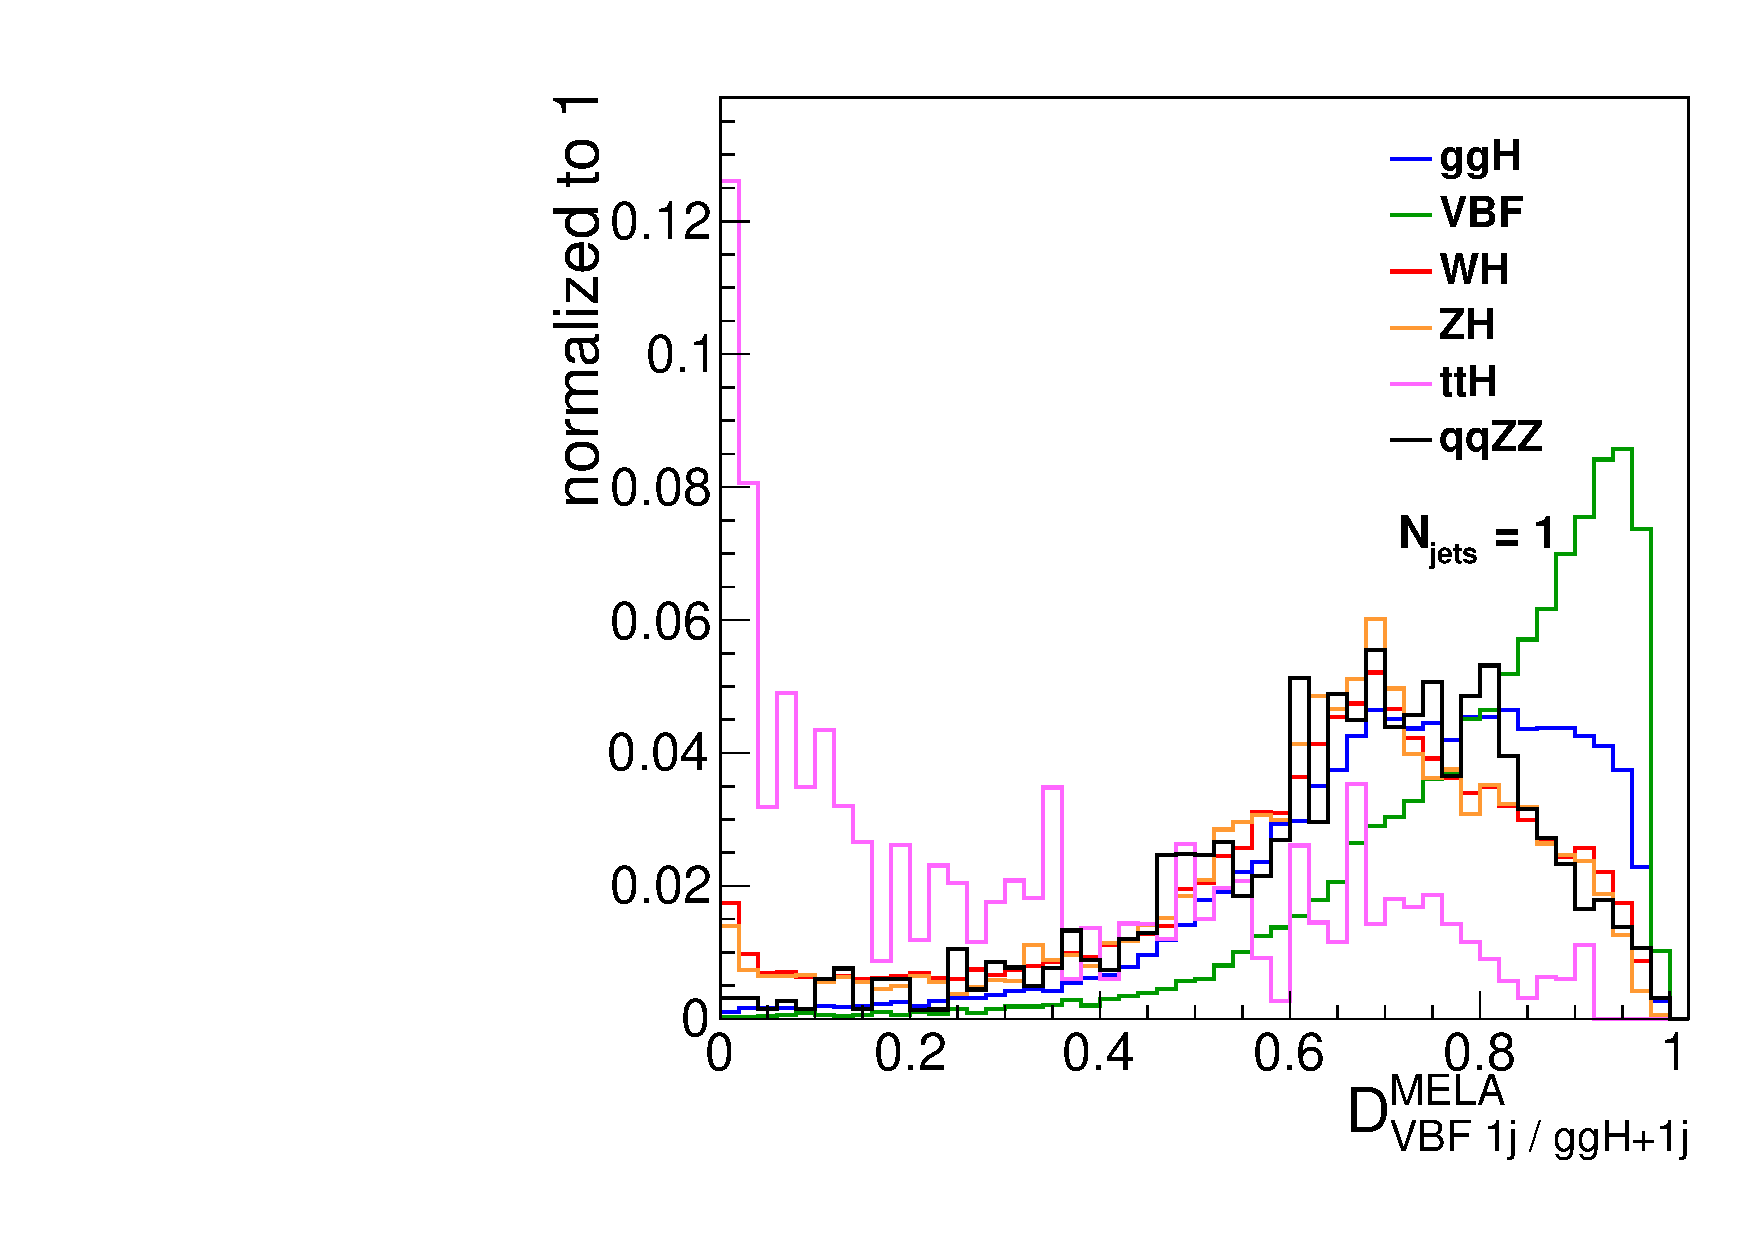
\includegraphics[width=0.45\textwidth]{Figures/Observables/cBCInSR_D1jVbfHj_m4l118to130_bList10_.pdf}
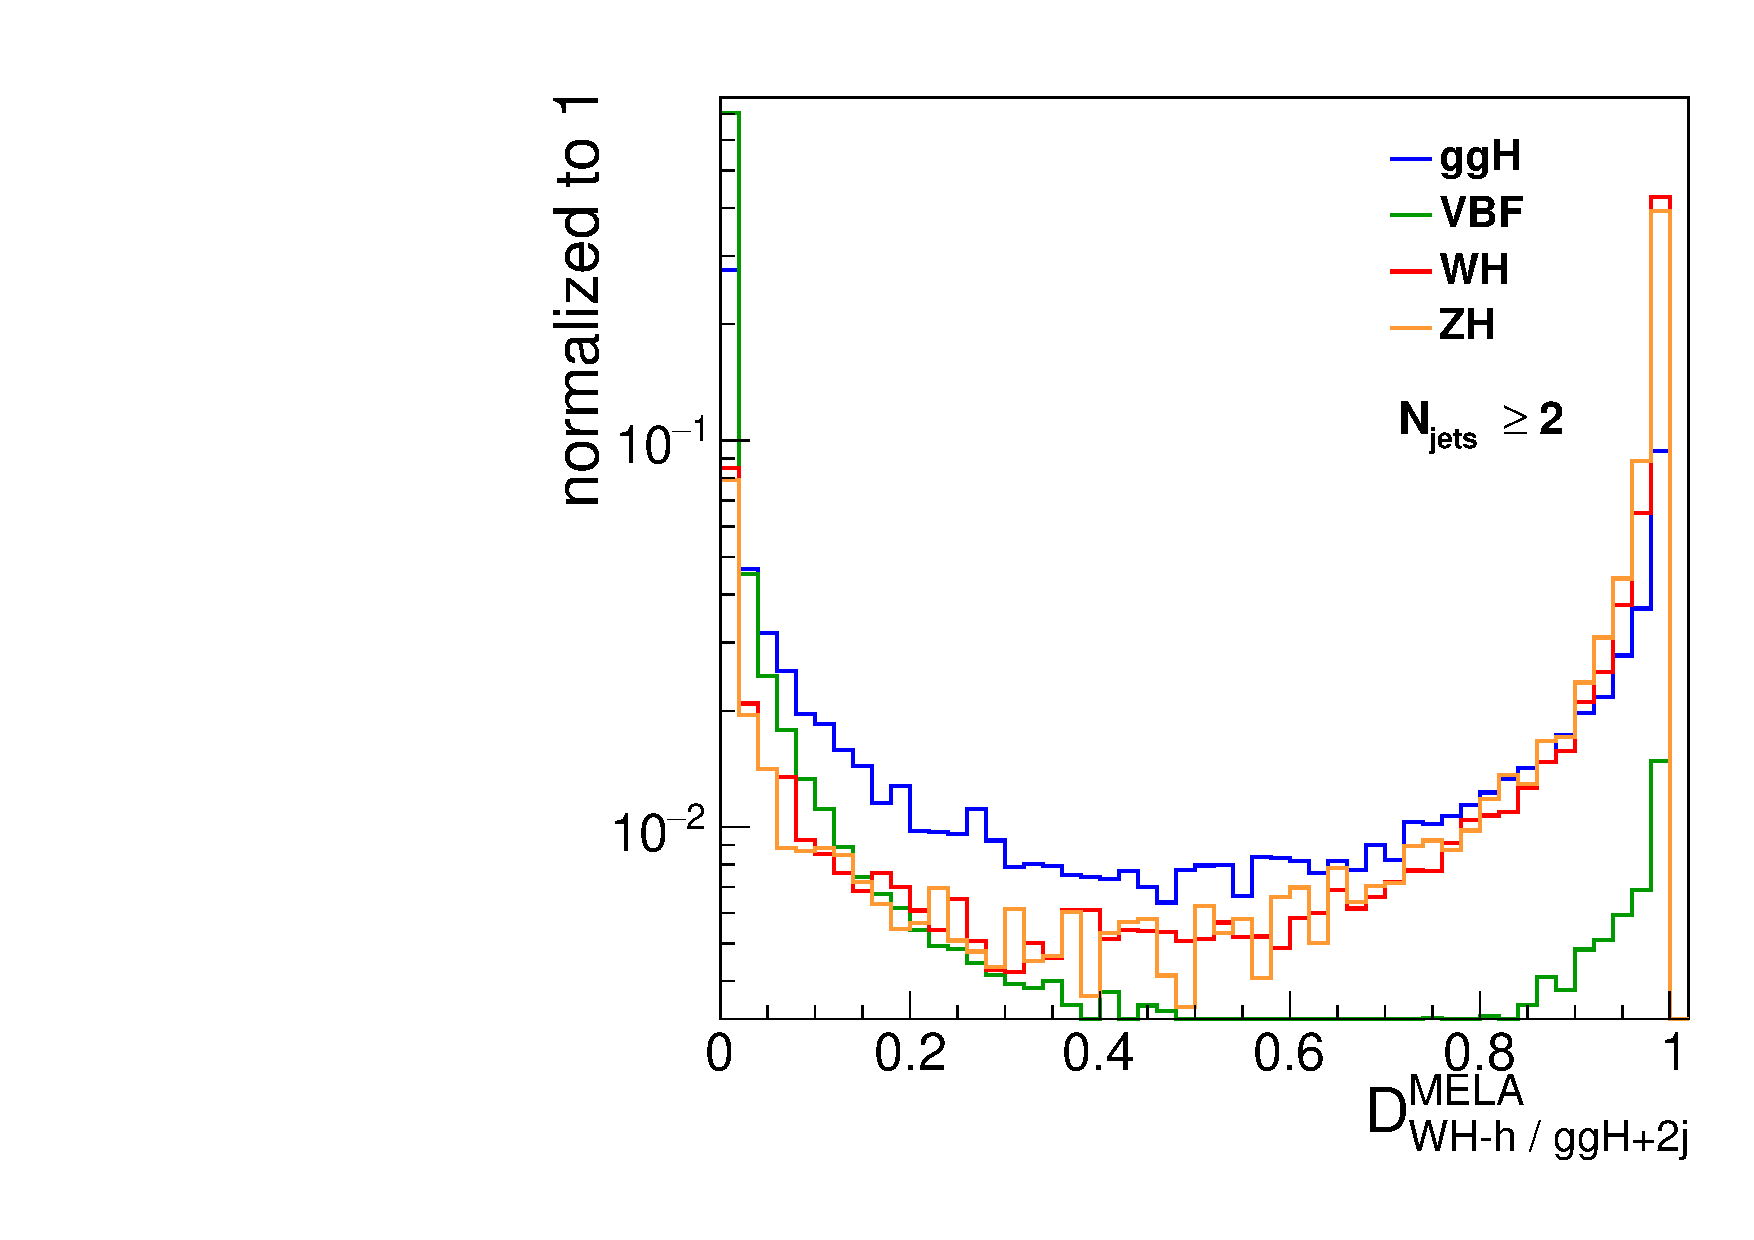
\includegraphics[width=0.45\textwidth]{Figures/Observables/cBCInSR_D2jWHHadrHjj_m4l118to130_bList10_.pdf}
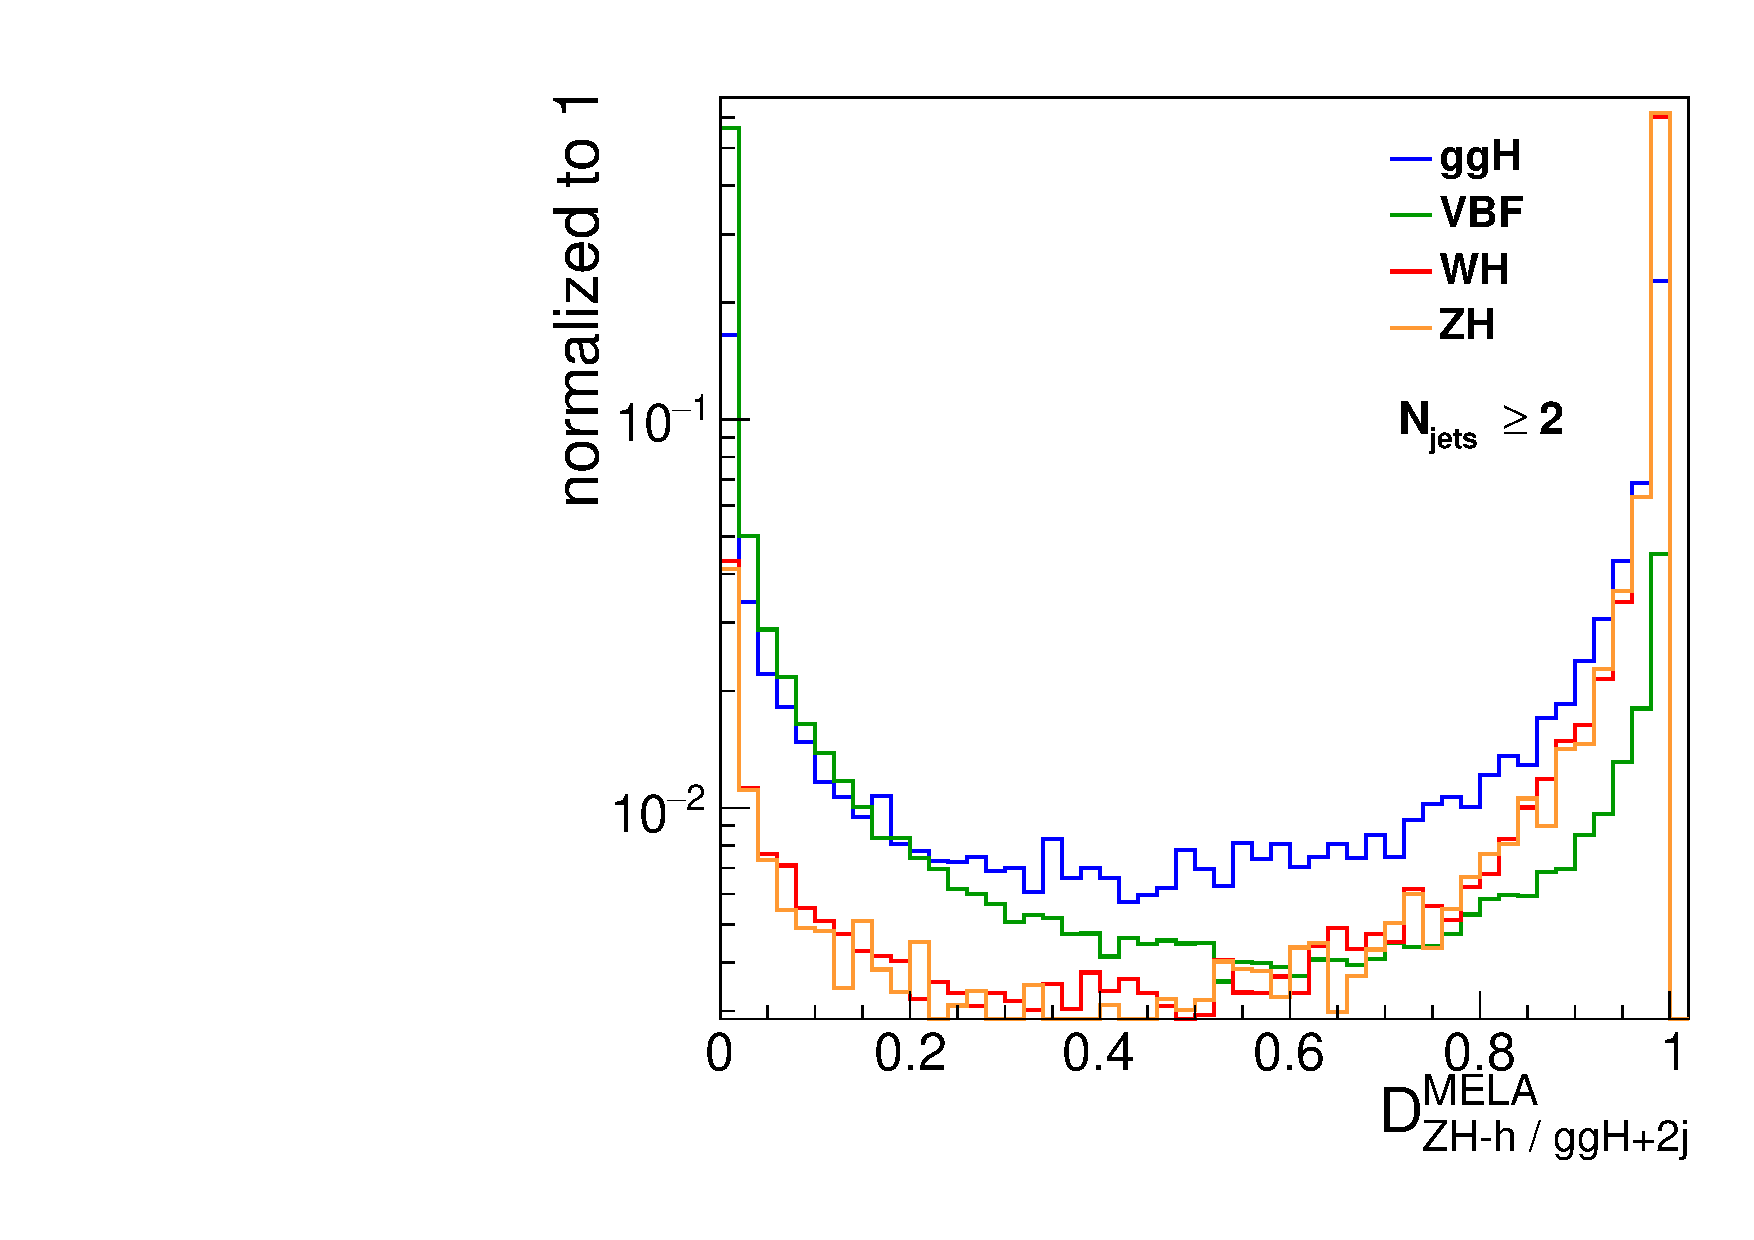
\includegraphics[width=0.45\textwidth]{Figures/Observables/cBCInSR_D2jZHHadrHjj_m4l118to130_bList10_.pdf}
\caption
{
Distribution of the 
\DMeVbfjj (top left),
\DMeVbfj (top right),
\DMeWh (bottom left),
\DMeZh (bottom right) 
discriminant for various production mechanisms of the H(125) signal and background
in the $H\to 4\ell$ analysis. MC simulation at 13 TeV is shown.
\label{fig:melaVBFVH}
}
\end{center}
\end{figure}
%=============                          

%Distribution of the $\mathcal{D}_{\rm jet}$ discriminant in most of the relevant 
%signal and background processes is shown in Fig.~\ref{fig:djet}.
%The input observables characterize the full kinematics of the VBF process, as indicated in Fig.~\ref{fig:decay} (right),
%at leading order in QCD. The observables include the invariant masses of the Higgs boson and of the two intermediate
%vector bosons in VBF production, as well as three angles 
%$\vec\Omega^{\rm \PH+JJ}$=($m_{4\ell}$, $q_1^2$, $q_2^2$, $\theta_1^{\textsc{vbf}}$, $\theta_2^{\textsc{vbf}}$, $\Phi^{\textsc{vbf}}$).
%The two angles  $\theta^{*\textsc{vbf}}$ and $\Phi_1^{\textsc{vbf}}$ are flat for both processes and provide no separation.
%The transverse momentum of the $HJJ$ system is left out of this calculation because it depends on NLO effects in QCD.
%Most of the observables historically used for VBF separation, such as di-jet invariant mass, can be calculated 
%using the above eight mass and angular observables.
%
%The idea of the $\mathcal{D}_{\rm jet}$ discriminant is identical to the idea of the original 
%MELA discriminant $\mathcal{D}_\text{bkg}^\text{kin}$ used for the Higgs boson discovery~\cite{Chatrchyan:2012ufa}, 
%with the difference that it explores full production kinematics at LO instead of only the decay kinematics at LO. 
%Both discriminants rely on the SM expectations for the HVV vertex. 
%It has been shown in the supporting documentation of Refs.~\cite{Khachatryan:2015cwa, Khachatryan:2015mma} 
%(CMS internal analysis notes) that $\mathcal{D}_{\rm jet}$ observable defined in Eq.~(\ref{eq:vbfmela}) has superior
%performance with respect to linear discriminants (such as fisher or $m_{JJ}$) and identical to the machine trained techniques 
%(such as BDT) when the same full information about the process is utilized in the input. However, the $\mathcal{D}_{\rm jet}$
%discriminant based on the matrix element has the advantage that it does not require training on MC samples, avoids potential
%overtraining bias, and appears to be reproducible for the outside world. It is also guaranteed to use the full kinematic
%information about the process and can be easily adjusted to other applications. 


%=============
%\begin{figure}[!htb]
%\vspace*{0.3cm}
%\begin{center}
%\includegraphics[width=0.45\textwidth]{Figures/Djet.pdf}
%\caption
%{ 
%Distribution of the $\mathcal{D}_{\rm jet}$ discriminant in most of the relevant 
%signal and background processes (listed in the legend) in the low-mass range around 125 GeV.
%MC simulation at 13 TeV is shown. 
%\label{fig:djet}
%}
%\end{center}
%\end{figure}
%=============

%Similar configurations exist for the production discriminant sensitive to the $V\PH$ and $t\bar{t}\PH$ signal topologies,
%as will be described in detail later. 

%================================================

% NO Q/G Discriminant used for now...
%
%In addition to matrix elements, further independent discriminating information can be obtained from quark-gluon tagging, since jets produced in association with gluon fusion are typically gluon-induced, while pairs of jets from VBF and VH processes are quark-induced.
%The quark-gluon tagger that is provided for 13\TeV analyses combines information from three input variables: $mult$ (jet particle multiplicity), $axis2$ (minor axis of the jet ellipse on the $\eta-\phi$ plane), and  $\pt D$ (jet fragmentation function).
%Global pdf's for light quarks ($\mathcal{Q}$) and gluons ($\mathcal{G}$) are defined as the products of light quark or gluon pdf's of these three variables. We use the 80X v0 version of the database, which relies on training samples from the RunIISpring16 production (CMSSW\_8\_0\_X reconstruction). 
%$\mathcal{Q}$ and $\mathcal{G}$ are used to build likelihood discriminants, the one-jet version of which reads:
%%%%%%%%%%%%%%%%%%%%%
%\begin{eqnarray}
%\label{eq:qg1j}
%\DQgj \equiv 
%\left[1+\frac{ \mathcal{G}(\mathrm{J})}{\mathcal{Q}(\mathrm{J})}\right]^{-1}
%\end{eqnarray}
%%%%%%%%%%%%%%%%%%%%% 
%where $\mathrm{J}=(mult, axis2, \pt D)$ denotes the set of input variables of a given jet.
%\DQgj can be used to discriminate gluon fusion events and VBF events that have exactly one selected jet. 
%To extract VBF or VH events with two associated jets, the following version is built:
%%%%%%%%%%%%%%%%%%%%%
%\begin{eqnarray}
%\label{eq:qg2j}
%\DQgjj \equiv 
%\left[1+\frac{ \mathcal{G}(\mathrm{J}_1) \mathcal{G}(\mathrm{J}_2)}{\mathcal{Q}(\mathrm{J}_1)\mathcal{Q}(\mathrm{J}_2)}\right]^{-1}\ ,
%\end{eqnarray}
%%%%%%%%%%%%%%%%%%%%%
%where $\mathrm{J}_1$ and $\mathrm{J}_2$ stand for the two highest-\pt selected jets.


% %=======
% \begin{figure}[!htb]
% \vspace*{0.3cm}
% \begin{center}
% \includegraphics[width=0.45\linewidth]{Figures/Observables/cCompareRocs_VBF2j_transform_m4l118to130_.pdf}
% \includegraphics[width=0.45\linewidth]{Figures/Observables/cCompareRocs_VBF1j_transform_m4l118to130_.pdf} \\
% \includegraphics[width=0.45\linewidth]{Figures/Observables/cCompareRocs_WHhadr_transform_m4l118to130_.pdf}
% \includegraphics[width=0.45\linewidth]{Figures/Observables/cCompareRocs_ZHhadr_transform_m4l118to130_.pdf}
% \caption{ROC curve comparisons of production discriminants used to extract four different processes from gluon fusion: VBF with two associated jets (top left), VBF with one associated jet (top right), \WH and \ZH with two associated jets (bottom left and right). Signal region events in a $105<\mllll<140\GeV$ window are used. Each plots compares MELA-based discriminants (green), quark-gluon discriminants (blue), combinations of both methods (red) and three transformed versions of the latter (shades of pink). Colored markers indicate the finally chosen discriminants and corresponding operating points used in event categorization (green: MELA-only categorization, pink: categorization combining MELA and quark-gluon tagging).
% \label{fig:prodtaggerROCs}}
% \end{center}
% \end{figure}
% %=======

% Information from matrix-element and quark-gluon discriminants can be condensed into combined discriminants by multiplying probability ratios from the above formulas, for instance
% $\left[1+\frac{ \mathcal{P}_{\rm HJJ} (\vec\Omega^{\rm \PH+JJ} | \mllll) }{\mathcal{P}_{\rm VBF}  (\vec\Omega^{\rm \PH+JJ} | \mllll)} \times \frac{ \mathcal{G}(\mathrm{J}_1) \mathcal{G}(\mathrm{J}_2)}{\mathcal{Q}(\mathrm{J}_1)\mathcal{Q}(\mathrm{J}_2)} \right]^{-1}$ 
% to separate VBF from gluon fusion in two-jet events.
% Nevertheless, such a variable is found to not perform as good as the MELA-based \DMeVbfjj alone, mostly because of internal correlations within $\mathcal{Q}$ and $\mathcal{G}$, which are not probabilities but products of three correlated probabilities.
% In order to bypass this behaviour, monotonic functions can be applied to the $\mathcal{G}/\mathcal{Q}$ ratios to give them less weight in the combined tagger. A variety of $x \longmapsto x^{1/n}$ fractional exponent functions were tested, three of which (square, cubic and quartic root) are illustrated in the ROC curves of Fig.~\ref{fig:prodtaggerROCs} and compared to the matrix-element-only and quark-gluon-only discriminants. Such transformations are found to not only improve the discrimination of VBF from gluon fusion in two-jet events, but also in 1-jet events, as well as discrimination of \WH and \ZH from gluon fusion in two-jet events.
% In all four cases, we choose to consistently apply the cubic root function to the quark-gluon factor of the combined discriminants, which are thus defined as follows:
%   %%%%%%%%%%%%%%%%%%%%%
%   \begin{eqnarray}
%   \label{eq:dcombvbf2j}
%   \DCombVbfjj \equiv 
%   \left[1+ 
%     \frac{ \mathcal{P}_{\rm HJJ} (\vec\Omega^{\rm \PH+JJ} | m_{4\ell}) }{\mathcal{P}_{\rm VBF}  (\vec\Omega^{\rm \PH+JJ} | m_{4\ell})  }
%     \times \left(\frac{ \mathcal{G}(\mathrm{J}_1) \mathcal{G}(\mathrm{J}_2)}{\mathcal{Q}(\mathrm{J}_1)\mathcal{Q}(\mathrm{J}_2)}\right)^{1/3} 
%     \right]^{-1}
%   \,, \\
%   \label{eq:dcombvbf1j}
%   \DCombVbfj \equiv 
%   \left[1+
%     \frac{ \mathcal{P}_{\rm HJ} (\vec\Omega^{\rm \PH+J} | m_{4\ell}) }{\int d\eta_{\rm J}\mathcal{P}_{\rm VBF}  (\vec\Omega^{\rm \PH+JJ} | m_{4\ell})  }
%     \times  \left(\frac{ \mathcal{G}(\mathrm{J})}{\mathcal{Q}(\mathrm{J})}\right)^{1/3} 
%     \right]^{-1}
%   \,,\\
%   \label{eq:dcombwh}
%   \DCombWh \equiv 
%   \left[1+
%     \frac{ \mathcal{P}_{\rm HJJ} (\vec\Omega^{\rm \PH+JJ} | m_{4\ell}) }{\mathcal{P}_{\rm WH}  (\vec\Omega^{\rm \PH+JJ} | m_{4\ell})  }
%     \times  \left(\frac{ \mathcal{G}(\mathrm{J}_1) \mathcal{G}(\mathrm{J}_2)}{\mathcal{Q}(\mathrm{J}_1)\mathcal{Q}(\mathrm{J}_2)}\right)^{1/3}
%     \right]^{-1}
%   \,,\\
%   \label{eq:dcombzh}
%   \DCombZh \equiv 
%   \left[1+
%     \frac{ \mathcal{P}_{\rm HJJ} (\vec\Omega^{\rm \PH+JJ} | m_{4\ell}) }{\mathcal{P}_{\rm ZH}  (\vec\Omega^{\rm \PH+JJ} | m_{4\ell})  }
%     \times  \left(\frac{ \mathcal{G}(\mathrm{J}_1) \mathcal{G}(\mathrm{J}_2)}{\mathcal{Q}(\mathrm{J}_1)\mathcal{Q}(\mathrm{J}_2)}\right)^{1/3}
%     \right]^{-1}
%   \,.
%   \end{eqnarray}
%   %%%%%%%%%%%%%%%%%%%%%

These discriminants are used to enhance the purity of the categories described in Section~\ref{sec:categorization}. Operating points then are defined, both for the 4 MELA-only discriminants and the 4 combined discriminants, so as to obtain a good compromise between expected category yields and purities. %Both sets of operating points are also illustrated in Fig.~\ref{fig:prodtaggerROCs}.

%================================================












